% Retoca las líneas marcadas con TODO según las necesidades

\documentclass[oneside,a4paper,12pt]{book} % TODO: cambia "oneside" por "twoside" a la hora de imprimirlo

\usepackage[spanish]{babel}
\usepackage[utf8]{inputenc}
\usepackage{geometry}
\usepackage{makeidx}
\usepackage{url}
\usepackage{graphicx}
\usepackage{color}
\usepackage{caption}
\usepackage{acronym}
\usepackage{hyphenat}
\usepackage{a4wide}
\usepackage[normalsize]{subfigure}
\usepackage{float}
\usepackage{titlesec}
\usepackage[Lenny]{fncychap}
\usepackage{listings} % para poder hacer uso de "listings" propios (p.ej. códigos)
\usepackage{eurosym} % para poder usar el símbolo del euro con \euro {xx}
\usepackage{hyperref} % TODO: añade la opción hidelinks para imprimirlo (los enlaces no aparecerán resaltados)
% EXPRESIONES MATEMÁTICAS
\usepackage{amsmath,amssymb,amsfonts,amsthm}
% Para que no parta las palabras
\pretolerance=10000

\usepackage{afterpage}
\newcommand\blankpage{%
    \null
    \thispagestyle{empty}%
    \addtocounter{page}{-1}%
    \newpage}

\newcommand{\bigrule}{\titlerule[0.5mm]} \titleformat{\chapter}[display] % cambiamos el formato de los capítulos
{\bfseries\Huge} % por defecto se usaron caracteres de tamaño huge en negrita
{% contenido de la etiqueta 
\titlerule % línea horizontal 
\filright % texto alineado a la derecha 
\Large\chaptertitlename\ % capítulo e índice en tamaño large
\Large % en lugar de 
\Huge \Large\thechapter} 
{0mm} % espacio mínimo entre etiqueta y cuerpo
{\filright} % texto del cuerpo alineado a la derecha
[\vspace{0.5mm} \bigrule] % después del cuerpo, dejar espacio vertical y trazar línea horizontal gruesa
\geometry{a4paper, left=3.5cm, right=2cm, top=3cm, bottom=2cm, headsep=1.5cm}

% Estilos para ilustrar códigos:
\definecolor{code_green}{rgb}{0,0.6,0}
\definecolor{code_gray}{rgb}{0.5,0.5,0.5}
\definecolor{code_mauve}{rgb}{0.58,0,0.82}

\lstset{frame=tb,
  language=C,
  aboveskip=3mm,
  belowskip=3mm,
  showstringspaces=false,
  columns=flexible,
  basicstyle={\small\ttfamily},
  numbers=none,
  numberstyle=\tiny\color{code_gray},
  keywordstyle=\color{blue},
  commentstyle=\color{code_green},
  stringstyle=\color{code_mauve},
  breaklines=true,
  breakatwhitespace=true,
  tabsize=3
}

\lstset{frame=tb,
  language=C++,
  aboveskip=3mm,
  belowskip=3mm,
  showstringspaces=false,
  columns=flexible,
  basicstyle={\small\ttfamily},
  numbers=none,
  numberstyle=\tiny\color{code_gray},
  keywordstyle=\color{blue},
  commentstyle=\color{code_green},
  stringstyle=\color{code_mauve},
  breaklines=true,
  breakatwhitespace=true,
  tabsize=3
}

\lstset{frame=tb,
  language=Python,
  aboveskip=3mm,
  belowskip=3mm,
  showstringspaces=false,
  columns=flexible,
  basicstyle={\small\ttfamily},
  numbers=none,
  numberstyle=\tiny\color{code_gray},
  keywordstyle=\color{blue},
  commentstyle=\color{code_green},
  stringstyle=\color{code_mauve},
  breaklines=true,
  breakatwhitespace=true,
  tabsize=3
}

% Definición de mis propios tipos: Códigos, Ecuaciones y Tablas
\DeclareCaptionType{code}[Código][Listado de códigos]
\DeclareCaptionType{myequation}[Ecuación][Listado de ecuaciones]

% TODO: especifica las reglas de separación que consideres. Algunos ejemplos:
\hyphenation{fuer-tes}
\hyphenation{mul-ti-ca-pa}
\hyphenation{res-pues-ta}
\hyphenation{di-fe-ren-tes}
\hyphenation{de-sa-rro-lla-dos}
\hyphenation{re-pre-sen-tan-do} % archivo de configuracion de estilo

\usepackage{array}
\usepackage{multirow}
\usepackage{natbib}

\hypersetup{
    colorlinks=true,
    linkcolor=black,
    urlcolor=black,
    citecolor=black
}

\makeindex

\begin{document}
\baselineskip 1.35\baselineskip

\frontmatter

\thispagestyle{empty}

\begin{titlepage}
	\begin{center}
		\vspace*{3mm}
		\begin{center}
			
\includegraphics[width=0.4\linewidth]{imagenes/cap1/logo_urjc}
		\end{center}
		\vspace{6.0mm}
		
		\fontsize{15.5}{14}\selectfont ESCUELA DE INGENIERÍA DE FUENLABRADA
		\vspace{13mm}
		
		\fontsize{14}{14}\selectfont GRADO EN INGENIERÍA DE ROBÓTICA SOFTWARE
		
		\vspace{70pt}
		
		\fontfamily{lmss}\fontsize{15.7}{14}\selectfont \textbf{TRABAJO FIN DE GRADO} 
		
		\vspace{20mm}
		\begin{LARGE}
			Navegación autónoma de un dron

			para localizar un transmisor de radio frecuencia
			
			basado en aprendizaje por refuerzo
		\end{LARGE}
		
		\vspace{20mm}
		
		\begin{large}
			Autor: Cristian Sánchez Rodríguez
			
			Tutor: Dr. Roberto Calvo Palomino
			
			\vspace{10mm}
		\end{large}
		\begin{normalsize}
			Curso académico 2023/2024		
		\end{normalsize}
		\vspace{10mm}
		
	\end{center}
	
\end{titlepage}

\thispagestyle{empty}


\cleardoublepage

\chapter*{Agradecimientos}

ToDo
\

\

\

\

\begin{flushright}
		\par
		\vspace{1.0 cm}
		Madrid, 30 de junio de 2023\\ %\today
		\emph{Cristian Sánchez Rodríguez}
\end{flushright}

\thispagestyle{empty}



\cleardoublepage

\chapter*{Resumen\markboth{Resumen}{Resumen}}

En la actualidad, la ciencia ha avanzado a pasos agigantados con respecto a las soluciones tecnológicas. Especialmente la robótica, también gracias a que abarca una inmensa variedad de campos donde se pueden desarrollar soluciones eficientes y robustas.\\

Además, ha surgido un nuevo paradigma con el uso de drones, o sistemas aéreos provistos de sensores y actuadores, que amplian el espectro de uso para herramientas tecnológicas, permitiendo abordar los problemas desde nuevas perspectivas. En este proyecto, el foco de estudio se centra en los \ac{UAV}, ya que se busca automatizar todo el proceso de manejo del mismo.\\

De este modo, surge la idea de realizar este \ac{TFG}, juntando lo mejor de ambos mundos, soluciones autónomas con dispositivos aéreos tremendamente adaptables a las circunstancias del problema.\\

Concretamente, el objetivo de este proyecto ha sido demostrar que, empleando aprendizaje por refuerzo (Q-Learning), se puede lograr rastrear y navegar hacia una señal \ac{RF} de forma más efectiva que con el resto de aproximaciones planteadas.

\cleardoublepage

\chapter*{Acrónimos\markboth{Acrónimos}{Acrónimos}}

% Añade a continuación los acrónimos que uses en el documento. Algunos ejemplos:
\begin{acronym}
	\acro{RAE}{Real Academia Española}
	\acro{TFG}{Trabajo de Fin de Grado}
	\acro{UAV}{\emph{Unmanned Air Vehicles}}
	\acro{UAS}{\emph{Unmanned Aerial Systems}}	
	\acro{GCS}{\emph{Ground Control Station}}
	\acro{SUAV}{\emph{Small Unmmaned Air Vehicle}}
	\acro{LOS}{\emph{Line Of Sight}}
	\acro{IA}{Inteligencia Artificial}
	\acro{RF}{Radio Frecuencia}
	\acro{EM}{Electromagnético}
	\acro{ROS}{\emph{Robot Operating System}}
	\acro{ADC}{\emph{Analog to Digital Converter}}
	\acro{RSSI}{\emph{Received Signal Strength Indicator}}
	\acro{SNR}{\emph{Signal to Noise Ratio}}
	\acro{PLE}{\emph{Path-Loss Exponent}}
	\acro{AMR}{\emph{Autonomous Mobile Robot}}
	\acro{AGV}{\emph{Automated Guided Vehicle}}
	\acro{SAR}{\emph{Search and Rescue}}
	\acro{VFF}{\emph{Virtual Force Field}}
	\acro{RL}{\emph{Reinforcement Learning}}
	\acro{MPSS}{Módulo de Propagación de Señal Simulado}
	\acro{ANAIV}{Algoritmo de Navegación Autónoma basado en la Información de la Vecindad}
	\acro{PPO}{\emph{Proximal Policy Optimization}}	
	\acro{DDPG}{\emph{Deep Deterministic Policy Gradient}}
	\acro{SAC}{\emph{Soft Actor Critic}}
\end{acronym}


\cleardoublepage

\tableofcontents

\listoffigures

\listofcodes

\listoftables

%\pagestyle{empty}

\cleardoublepage

 % aqui se cargan todas las "primeras paginas"

% Bibliografia
\let\OLDthebibliography=\thebibliography
\def\thebibliography#1{\OLDthebibliography{#1}
  \addcontentsline{toc}{chapter}{\bibname}}

\mainmatter

\setcounter{page}{1}
\chapter{Introducción}
\label{cap:capitulo1}
\setcounter{page}{1}

ToDo...

\section{Exoesqueletos}
\label{sec:exoesqueletos}

ToDo...

\subsection{Exoesqueletos en rehabilitación}
\label{subsec:exoesqueletos_rehabilitacion}

ToDo...

\section{Redes neuronales para detección de posturas}
\label{subsec:redes_neuronales_deteccion_posturas}

ToDo...

\chapter{Objetivos}
\label{cap:capitulo2}

En este capítulo se tratará el propósito de este proyecto, así como los requerimientos, el método seguido y la estructura del mismo.\\

\section{Descripción del problema}
\label{sec:descripcion_problema}

Los drones son una herramienta tremendamente versátil, ya que permiten solventar los inconvenientes orográficos de forma sencilla, y pueden ser provistos de múltiples sensores, lo que incrementa su adaptabilidad para solucionar un gran abanico de retos ingenieriles.\\

Por tanto, el foco de este \ac{TFG} consistirá en desarrollar un comportamiento autónomo en un dron, para detectar una señal \ac{RF}. Esto puede ser especialmente útil en labores de rastreo e identificación de objetivos, tales como en casos de escenarios catastróficos donde se deben localizar personas perdidas.\\

Para ello, se establecen los siguientes objetivos:

\begin{enumerate}
	\item Desarrollo de una aplicación, enfocada a teleoperar un cuadracóptero, empleando herramientas de simulación y visualización así cómo el tratamiento del código.
	\item Implementación de un modelo sencillo de propagación de señales.
	\item Desarrollo de un comportamiento autónomo capaz de identificar y navegar hacia una señal \ac{RF}.
	\item Comparativa frente a los algoritmos navegación tradicionales.
	\item Desarrollo de un comportamiento autónomo en un escenario con obstáculos.
\end{enumerate}

\section{Requisitos}
\label{sec:requisitos}

Las especificaciones que se deben cumplir son las siguientes:

\begin{enumerate}
	\item El modelo de propagación de señal debe ser el modelo de Friis.
	\item Se debe usar \ac{ROS} como middleware robótico y Gazebo como herramienta de simulación.
	\item Se debe seleccionar el algoritmo que navegue de forma más óptima.
	\item Se debe seleccionar el algoritmo más seguro.
\end{enumerate}

\section{Metodología}
\label{sec:metodologia}

Este trabajo, comenzó oficialmente en Septiembre de 2022, aunqué se pusieran en común las ideas a principios del verano, y se concluye a finales de Septiembre de 2023.\\ 

La metodología para llevarlo a cabo fue la siguiente:

\begin{enumerate}
	\item Reunión de control semanal o cada dos semanas vía Teams con el tutor, donde se realizaba una valoración del estado del proyecto y se establecían los futuros puntos a seguir.
	\item Uso de la metodología Kanban, que es una metodología visual para gestionar y optimizar el flujo de trabajo a través de tarjetas y límites de trabajo en curso.
	\item Empleo de la plataforma Github, a fin de establecer un repositorio común\footnote[1]{\url{https://github.com/RoboticsLabURJC/2022-tfg-cristian-sanchez}}, como sistema de control de versiones y de almacenamiento de backups.
	\item Desarrollo de un blog donde se describe el estado del proyecto\footnote[2]{\url{https://roboticslaburjc.github.io/2022-tfg-cristian-sanchez/}}.
\end{enumerate}

\begin{figure} [H]
	\begin{center}
	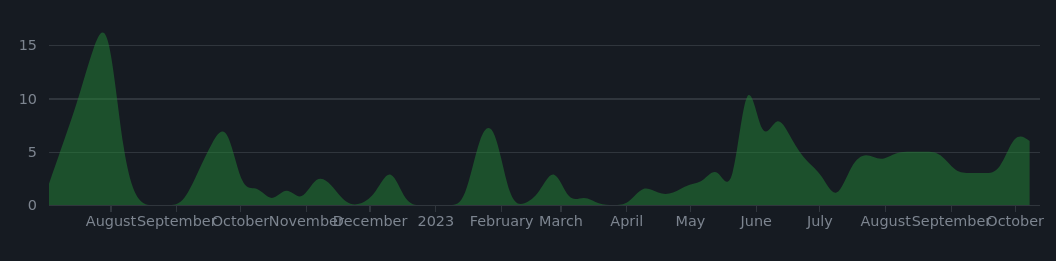
\includegraphics[height=3cm]{imagenes/cap2/1_insights.png}
	\end{center}
	\caption[Insights Github por meses \ac{TFG}]{Insights Github por meses \ac{TFG}}
	\label{fig:insights}
\end{figure}

\section{Plan de trabajo}
\label{sec:plantrabajo}

Para concluir este capítulo, los pasos seguidos han sido:

\begin{enumerate}
	\item Etapa inicial, donde tras establecer los objetivos del proyecto, se empezó por investigar el estado del arte del uso de drones para aplicaciones robóticas.
	\item Los primeros pasos en el \ac{TFG} se centrarón realizar una aplicación para teleoperar a un dron.
	\item El siguiente punto se basó en el estudio y comprensión de las señales \ac{RF} dentro del espectro de radiofrecuencia.
	\item Posteriormente, se desarrollaron diversas soluciones encargadas de resolver el problema de detectar y navegar hacia una señal.
	\item A continuación, se realizó una fase de pruebas y extracción de información sobre la que se realizaron diversas comparativas.
	\item Cerrando la fase de desarrollo, lo último fue implementar soluciones sobre escenarios más realistas que incluían obstáculos.
	\item Finalmente, se realizó la redacción de la memoria.
\end{enumerate}

\chapter{Plataformas de desarrollo y herramientas utilizadas}
\label{cap:capitulo3}

En este apartado se hablará de los recursos ingenieriles empleados para hacer posible el proyecto.

\section{Lenguajes de programación}
\label{sec:lenguajes_programacion}

\subsection{Python}
\label{subsec:python}

\begin{code}[hp]
	\begin{lstlisting}[language=Python]
	#! /usr/bin/env python
	
	if __name__ == "__main__":
		C = 3.0 * (10 ** 8)
		freq = 5 * (10 ** 9)
		lmbda = C / freq
	\end{lstlisting}
	\caption[Obtención del parámetro lambda en función de una frecuencia (en este caso 5G)]{Obtención del parámetro $\lambda$ en función de una frecuencia (en este caso 5G)}
	\label{cod:helloworld_python}
\end{code}

A día de hoy, es considerado el lenguaje de programación más popular \footnote[1]{\url{https://www.tiobe.com/tiobe-index/}}. Se ideó en 1991 por Guido van Rossum y se desarrolló en la Python Software Foundation \footnote[2]{\url{https://www.geeksforgeeks.org/history-of-python/}}. Es interpretado, es decir, usa un programa que traduce las líneas de código para la máquina en tiempo de ejecución (lo cual lo hace más intuitivo pero menos eficiente). Además, permite la programación orientada a objetos en alto nivel, lo que ofrece gran dinamismo a la hora de usarlo \footnote[3]{\url{https://www.python.org/doc/essays/blurb/} \url{https://www.educative.io/blog/compiled-vs-interpreted-language}}.\\

Debido a su amplia popularidad, podemos acceder a una gran variedad de módulos y utilidades desarrollados por la comunidad, los cuales se integran perfectamente en la resolución de nuestro problema.\\

En nuestro caso, python se usó para el crear la mayor parte del código empleado, es decir, para desarrollar interfaces gráficas, para trabajar con el middleware robótico \ac{ROS} (detallado posteriormente) y para el desarrollo de los diversos algoritmos. Todo ello haciendo uso del módulo \textbf{numpy}, el cual nos permite realizar operaciones matemáticas y trabajar con vectores de forma rápida y eficiente; así cómo del módulo \textbf{matplotlib}, del cual hablaremos más adelante.\\

\subsection{C++}
\label{subsec:cplusplus}

\begin{code}[hp]
	\begin{lstlisting}[language=C++]
	#include <iostream>
	
	int main(int argc, char ** argv) {
		std::cout << "Hello World!" << std::endl;
		return 0;
	}
	\end{lstlisting}
	\caption[Hello world en C++]{\emph{Hello world} en C++}
	\label{cod:helloworld_cplusplus}
\end{code}

También bastante popular, se encuentra el lenguaje de programación creado por Bjarne Stroustrup, en los laboratorios Bell en 1971. En este caso es compilado, lo que implica la traducción y enlazado previo a la ejecución. De corte más eficiente que Python, también permite la programación orientada a objetos. Se sitúa a medio camino entre un lenguaje de alto nivel y uno de bajo nivel \footnote[4]{\url{https://www.geeksforgeeks.org/history-of-c/}}.\\

El uso designado en este proyecto para este lenguaje fue para poder trabajar con mapas de calor, mediante la biblioteca de \emph{Anybotics} de grid maps\footnote[5]{\url{https://github.com/ANYbotics/grid_map}}.

\section{\ac{ROS}}
\label{sec:ros}

\begin{figure} [tp]
	\begin{center}
	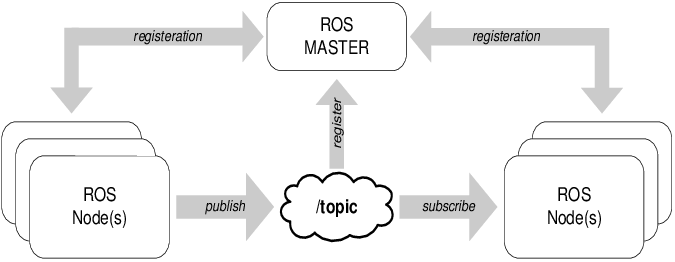
\includegraphics[height=4cm]{imagenes/cap3/1_ros_esquema.png}
	\end{center}
	\caption[Esquema de comunicaciones en ROS]{Esquema comunicaciones en ROS}
	\label{fig:ros}
\end{figure}

Si se habla de robótica, se habla de \ac{ROS}, ya que es el framework para el desarrollo de soluciones de este ámbito, pero, ¿qué es exactamente \ac{ROS}?.\\

Se trata de un \emph{middleware}, es decir, una infraestructura software situada entre el sistema operativo y el desarrollador, que incluye una serie de módulos y funcionalidades enfocadas al desarrollo de aplicaciones robóticas \footnote[6]{\url{https://www.ibm.com/topics/middleware} \url{https://www.ros.org/}}. La idea detrás, busca estandarizar soluciones que no dependan de los drivers de cada sensor y actuador presentes. De forma general, se trata de una arquitectura basada en el paradigma de publicador-suscriptor, donde una serie de nodos se comunican entre sí, transmitiendo mensajes propios, a través de canales compartidos llamados \emph{topics}, esto es, un nodo suscriptor se suscribirá a un determinado topic, que permita la transmisión de un tipo de mensaje concreto, quedando en espera de que un nodo pulicador, envíe mensajes de este tipo a ese topic, tal y como se puede apreciar en la figura~\ref{fig:ros}.\\

Concretamente, se usa para desarrollar todos los algoritmos robóticos y para realizar las comunicaciones necesarias en la simulación del dron.\\

\subsection{Rviz}
\label{subsec:rviz}

\begin{figure} [t]
	\begin{center}
	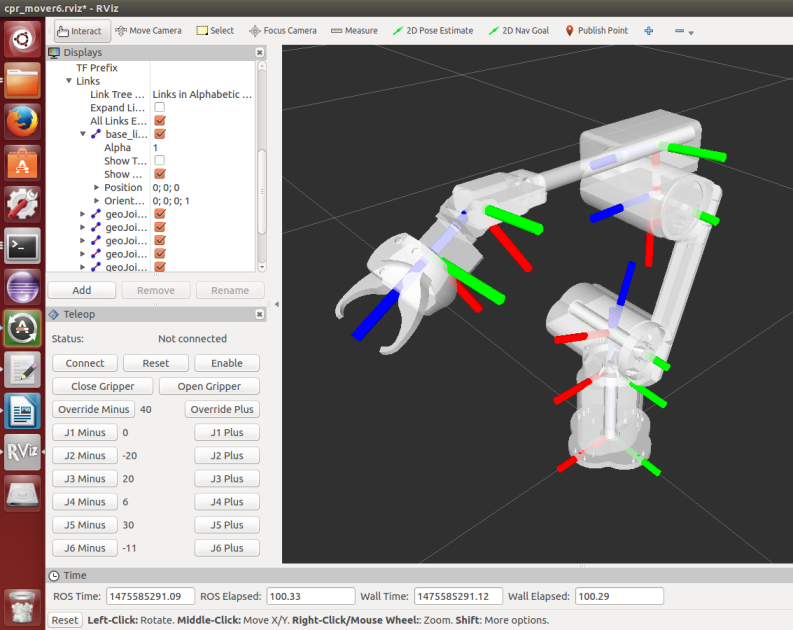
\includegraphics[height=10cm]{imagenes/cap3/3_rviz_example.png}
	\end{center}
	\caption[Ejemplo de uso de Rviz]{Ejemplo de uso de Rviz}
	\label{fig:rviz}
\end{figure}

Es un visualizador 3D diseñado para la depuración de aplicaciones \ac{ROS} \footnote[7]{\url{https://github.com/ros-visualization/rviz}}, tal y como se puede ver en la figura~\ref{fig:rviz}.\\

En nuestro caso, nos permite ver como se dispersa la señal \ac{RF}, que trayectoria y orientación sigue el dron, que efecto tiene sobre la señal la presencia de obstáculos, y otras tantas opciones.\\

\section{Gazebo 11}
\label{sec:gazebo}

\begin{figure} [t]
	\begin{center}
	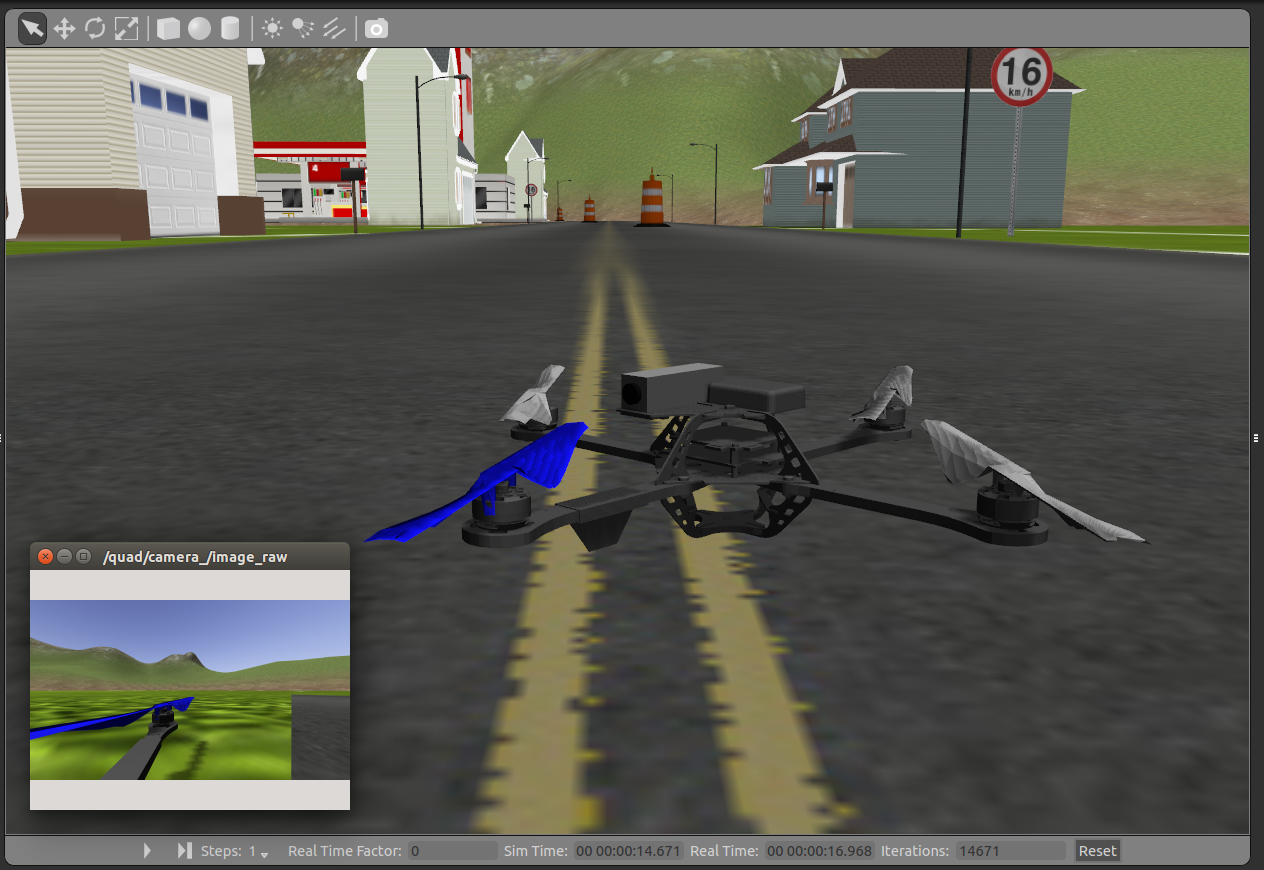
\includegraphics[height=10cm]{imagenes/cap3/2_gazebo_drone.png}
	\end{center}
	\caption[Simulación dron en Gazebo]{Simulación dron en Gazebo}
	\label{fig:gazebo}
\end{figure}

Se trata del simulador sobre el cual se desarrolla el proyecto. Concretamente consta de un conjunto de módulos optimizados para desarrollar aplicaciones robóticas, ampliamente compatible con \ac{ROS} (ver figura~\ref{fig:gazebo}). Además, posee un motor de físicas basado en ODE, lo que permite simular con precisión el funcionamiento de un dron \footnote[8]{\url{https://gazebosim.org/about}}.\\

Esta herramienta, nos permite visualizar en directo, el comportamiento del dispositivo frente a los diversos escenarios que se planteen.

\section{Plataformas de programación}
\label{sec:plataformas_de_programacion}

\subsection{Visual Studio Code}
\label{subsec:visual_studio_code}

% \begin{figure} [hp]
% 	\begin{center}
% 	
\includegraphics[height=3cm]{imagenes/cap3/4_vscode_logo.png}
% 	\end{center}
% 	\caption[VS Code logo]{VS Code logo}
% 	\label{fig:vscode}
% \end{figure}

Entre las plataformas usadas para programar, \emph{Visual Studio Code}, o mejor conocido como \emph{VS code}, es un editor de código ligero, funcional tanto en Linux, Windows y macOS \footnote[9]{\url{https://code.visualstudio.com/docs}}.\\

Su principal ventaja, es que es altamente personalizable a el tipo de desarrollo software que se desee realizar. Todo ello a través de las múltiples extensiones que ofrece, así como la conexión directa y fluida con plataformas como Github, que se detallarán a continuación.\\

\subsection{Github}
\label{subsec:github}

Github nace de la herramienta git, creada por Linus Torvalds (desarrollador de Linux), que es un sistema de control de versiones, que funciona a grandes rasgos a través de repositorios (o lugares donde se almacenan los sistemas de versiones de forma local), y commits (que permiten actualizar la version del código almacenado del repositorio) \footnote[10]{\url{https://www.howtogeek.com/180167/htg-explains-what-is-github-and-what-do-geeks-use-it-for/}}.\\

De este modo, Github consiste en trasladar la idea de tener repositorios locales, para distribuirlos en una plataforma online, donde además se permita el desarrollo de aplicaciones de manera colaborativa.\\

Por ello, el papel que toma en este proyecto es de vital importancia, ya que asegura un seguimiento y una seguridad, de cara a tener copias de seguridad, donde todo el que desee puede acceder a ver en que punto se encuentra el \ac{TFG} pueda hacerlo.\\

\section{Módulos}
\label{sec:modulos}

\subsection{OpenCV}
\label{subsec:opencv}

\begin{figure} [t]
	\begin{center}
	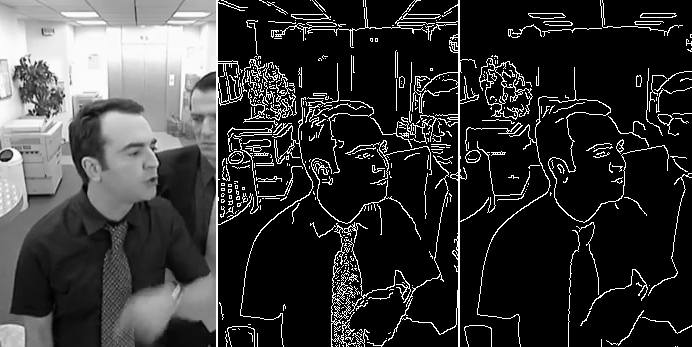
\includegraphics[height=8cm]{imagenes/cap3/5_opencv_example.png}
	\end{center}
	\caption[Interfaz gráfica usando OpenCV]{Interfaz gráfica usando OpenCV}
	\label{fig:opencv}
\end{figure}

Es una biblioteca software de python, enfocada a visión artificial, y que además dispone de otras funcionalidades útiles para el desarrollo \footnote[11]{\url{https://opencv.org/about/}}.\\

Por tanto, el uso designado en este proyecto es el de implementar interfaces gráficas sencillas (vease el ejemplo de la figura~\ref{fig:opencv}), sobre las que interactuar dinámicamente con el dron, a través de barras de acción y botones.

\subsection{Matplotlib}
\label{subsec:matplotlib}

\begin{figure} [t]
	\begin{center}
	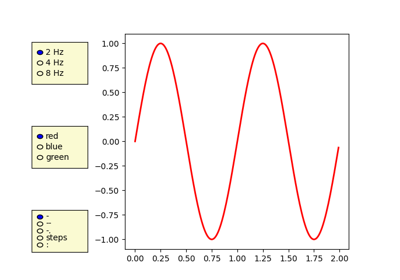
\includegraphics[height=7cm]{imagenes/cap3/6_matplotlib_app.png}
	\end{center}
	\caption[Representación de un mapa de calor usando matplotlib]{Representación de un mapa de calor usando matplotlib}
	\label{fig:matplotlib}
\end{figure}

Presentada por John Hunter en 2002, se usó como alternativa para el desarrollo de interfaces gráficas. La gran diferencia radica en que está diseñada para trabajar con estructuras numéricas del tipo array (muy compatible con Numpy \footnote[12]{\url{https://numpy.org/about/}}), lo que permite ofrecer una gran visualización y una interfaz responsiva \footnote[13]{\url{https://www.geeksforgeeks.org/python-introduction-matplotlib/}}.\\

Concretamente en este proyecto se usa para desarrollar implementar mapas de calor (que en definitiva son estructuras numéricas del tipo array), dentro de una interfaz gráfica (de forma similar a la representación de la figura~\ref{fig:matplotlib}), para simular el comportamiento de una señal \ac{RF}, permitiendo modificar los parámetros de la ecuación en tiempo real.

\subsection{PX4 autopilot}
\label{subsec:px4}

\begin{figure} [tp]
	\begin{center}
	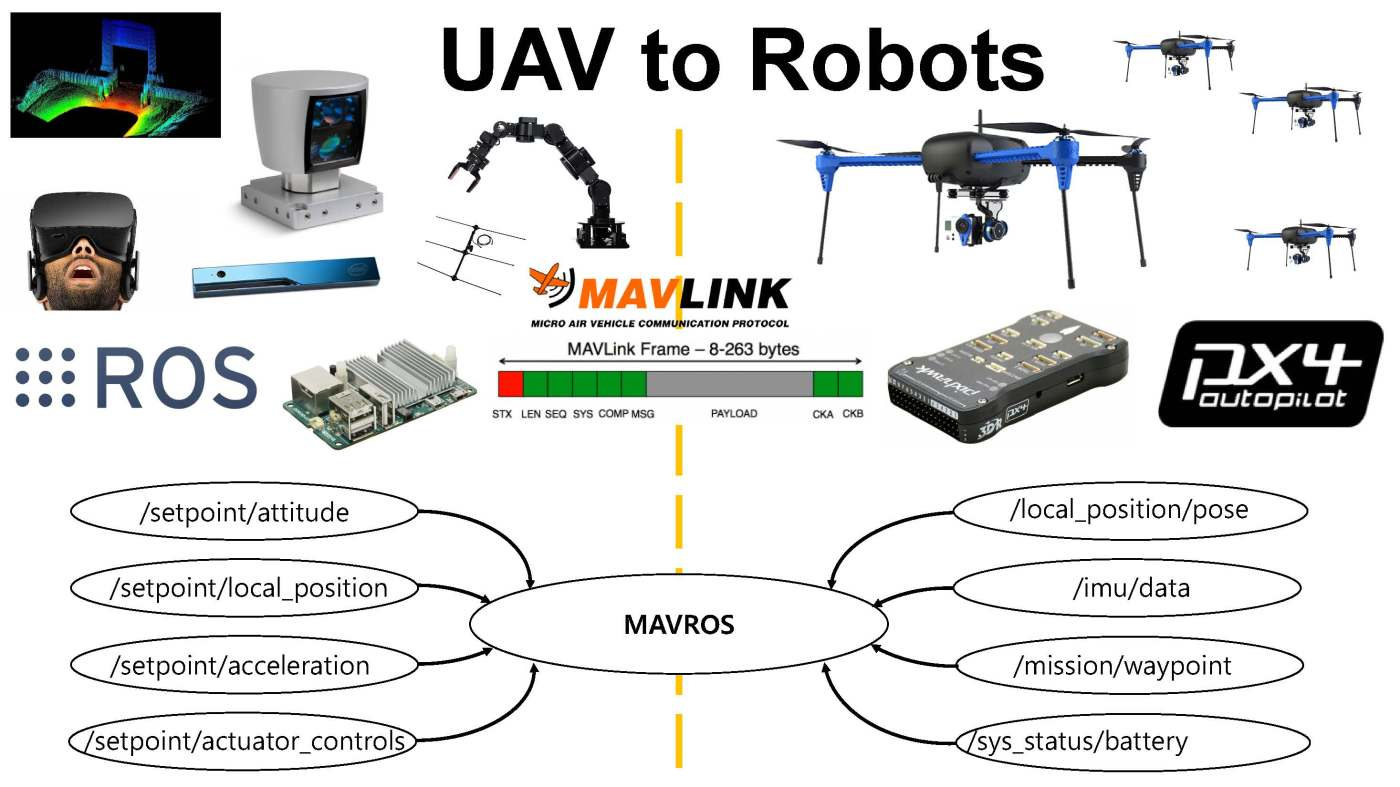
\includegraphics[height=6cm]{imagenes/cap3/7_px4_logo.jpeg}
	\end{center}
	\caption[Panorámica de PX4 con \ac{ROS}]{Panorámica de PX4 con \ac{ROS}}
	\label{fig:px4autopilot}
\end{figure}

Es la capa de software que permite hacer funcionar las aeronaves con sus componentes, esto es a través del controlador de vuelo, que a efectos prácticos se trata del cerebro del sistema, es decir, interconecta los sensores y actuadores, permitiendo comandar diversas acciones \footnote[14]{\url{https://www.droneblog.com/drone-controller/} \url{https://docs.px4.io/main/en/}}.\\

Este sistema, usa un conocido protocolo de comunicaciones llamado \textbf{MAVLink} (ver figura~\ref{fig:px4autopilot}), que se encarga de gestionar la comunicación entre el controlador de vuelo y la \ac{GCS}. En nuestro caso, y como queremos desarrollar aplicaciones mediante \ac{ROS}, debemos añadir una capa más, que se encarga de traducir los mensajes ROS a mensajes compatibles con el protocolo MAVLink, y de esto se encarga \textbf{MAVROS} \footnote[15]{\url{https://docs.px4.io/main/en/middleware/mavlink.html} \url{https://docs.px4.io/main/en/ros/ros1.html}}.\\

\begin{figure} [tp]
	\begin{center}
	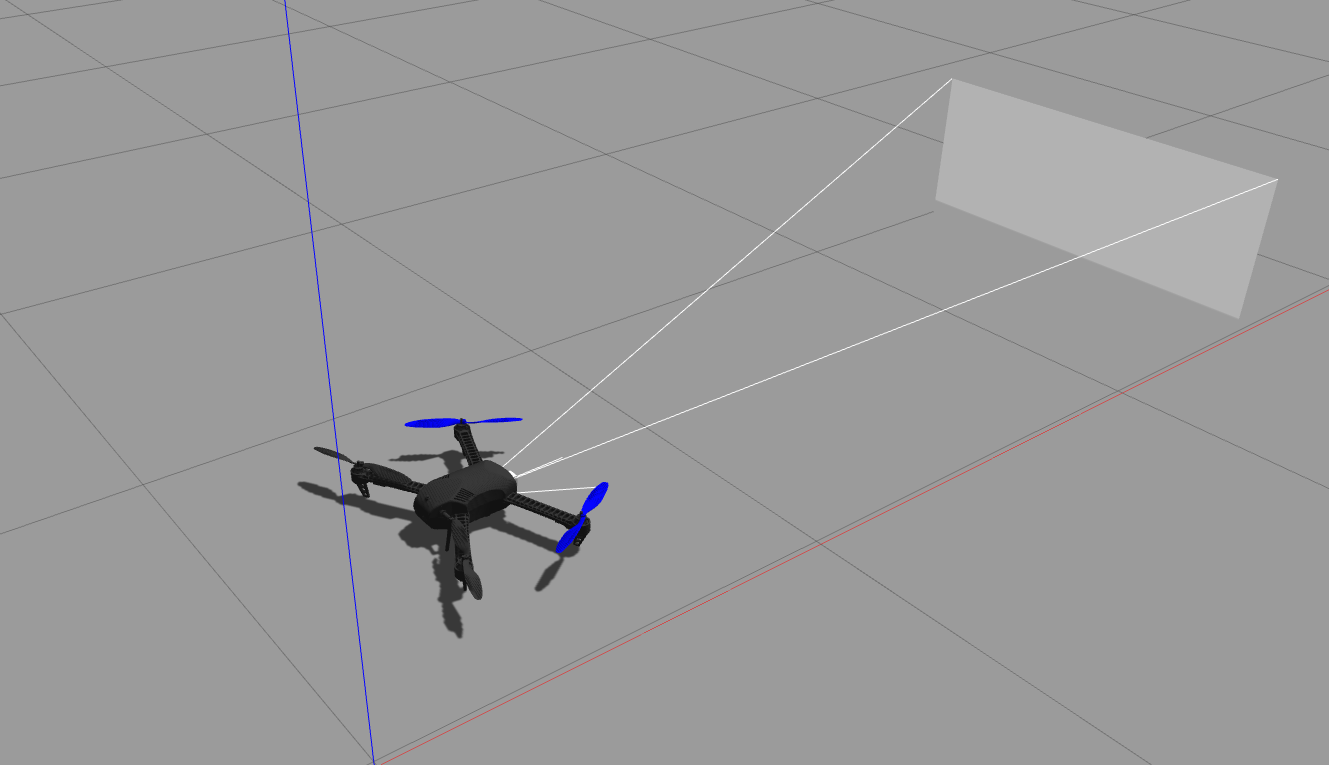
\includegraphics[height=5cm]{imagenes/cap3/8_iris_drone.png}
	\end{center}
	\caption[Iris drone en Gazebo 11]{Iris drone en Gazebo 11}
	\label{fig:irisdrone}
\end{figure}

\section{Iris}
\label{sec:iris}

Es el nombre de la aeronave representada en la figura~\ref{fig:irisdrone} y usada para solucionar los problemas planteados. En síntesis, es un dron cuadracóptero provisto de una cámara y un sensor de \ac{RF} simulado. Dicha aeronave es cortesía de \textbf{JdeRobot}, que es una organización sin ánimo de lucro, asociada a \emph{RoboticsLabURJC}, que provee de un conjunto de herramientas pensadas para desarrollar aplicaciones robóticas \footnote[16]{\url{https://jderobot.github.io/}}.\\

\chapter{Diseño}
\label{cap:capitulo4}

Tras haber puesto en contexto todo lo anterior, en este capítulo se expondrá, de forma detallada, el proceso seguido para conseguir que un dron detecte y navegue hacia una señal \ac{RF}.\\

Además, se mostrará el desarrollo de una aplicación responsiva, que simula el comportamiento de una señal (en un espacio libre de obstáculos), basada en la aproximación de Friis.\\

Por último, se buscará determinar cuál de los métodos empleados es mejor y por qué, a través de diversas métricas comparativas que se expondrán en detalle posteriormente.\\

\section{Preparación del entorno}
\label{sec:preparacion_del_entorno}

Lo primero que se debía conseguir, era un entorno de simulación compatible con \ac{ROS}, así como un sistema de control de versiones, que nos permitiera mantener la trazabilidad y los backups a mano. Por ello, se estableció un repositorio común en \textbf{GitHub} y se empleó el paquete de herramientas dispuesto por \textbf{JdeRobot}.

\subsection{JdeRobot - drones}
\label{subsec:jderobot_drones}

Gracias a esta plataforma, se pudieron obtener los modelos y los módulos necesarios para simular en Gazebo 11 el desempeño de un cuadracóptero, provisto de un sistema autopilot PX4.\\
\newpage
El modelo usado es el \textbf{3DR Iris simulado}, con un plugin de una cámara frontal. Este dispositivo utiliza MAVROS para realizar la comunicación, lo que nos permite enviar y recibir mesajes ROS compatibles con el protocolo de comunicaciones típico de estas aeronaves, MAVLink.\\

\begin{figure} [H]
	\begin{center}
	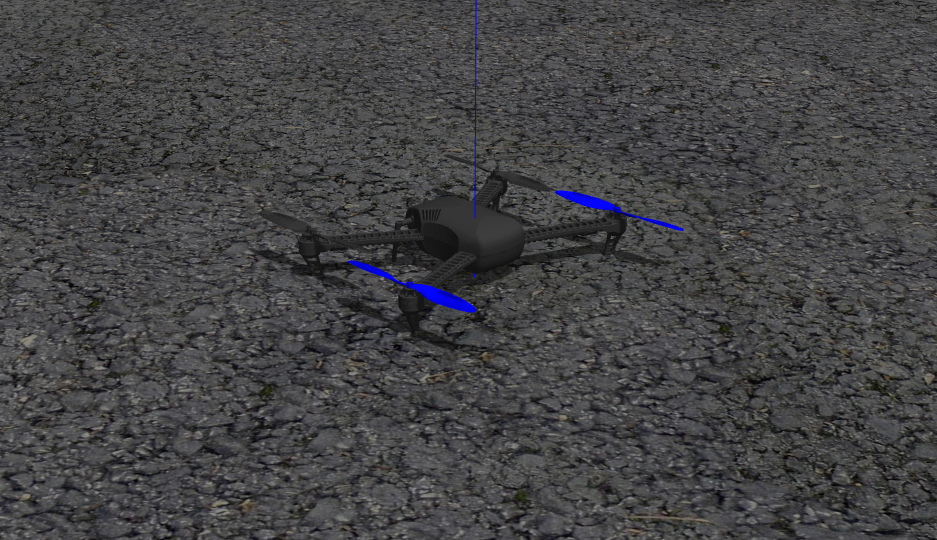
\includegraphics[height=4cm]{imagenes/cap4/1_px4_drone_gz.png}
	\end{center}
	\caption[3DR Iris simulado]{3DR Iris simulado}
	\label{fig:3dr_iris}
\end{figure}

\subsection{Teleoperador}
\label{subsec:teleoperador}

Ya propiamente hablando de resolver el problema planteado, la primera aproximación propuesta fue hacer una interfaz gráfica simple, que permitiera enviar órdenes a la aeronave.\\

Para ello, inicialmente se debía conseguir enviar mensajes de forma programática. Por tanto, se diseñó un \textbf{script controlador} encargado de la comunicación directa con el \textbf{controlador de la aeronave}, para enviar y recibir diversos datos vía MAVROS. De igual modo, se debían satisfacer una serie de requisitos que aseguraran el correcto funcionamiento del sistema:

\begin{enumerate}
	\item La comunicación debe darse a \textbf{más de 2Hz}, para evitar cambios indeseados en el funcionamiento interno del controlador PX4 (de la aeronave).

	\item Antes de realizar cualquier comunicación, \textbf{debe asegurarse que el estado es \emph{``connected''}}, lo que significa que el dron esta armado y en modo \emph{OFFBOARD} (nuestra aeronave posee 7 modos distintos, \emph{HOLD}, que mantiene la posición, \emph{RETURN}, que vuelve al punto de despegue, \emph{MISSION}, que permite cargar rutas programadas con anterioridad, \emph{TAKEOFF}, habilita el despegue, \emph{LAND}, habilita el aterrizaje, \emph{FOLLOW ME}, que permite seguir objetivos, y \emph{OFFBOARD}, que permite comandar al dron sin necesidad de GPS, lo que es útil de cara al desarrollo de aplicaciones robóticas) \cite{flight-modes}.

    \item Una vez esta conectado, se deben \textbf{enviar datos} (velocidades en nuestro caso) al controlador PX4, con el fin de \textbf{evitar el cierre de la conexión}. Estos datos carecen de utilidad más que la de asegurar dicha conectividad.

    \item Por último, y antes de enviar cualquier posición, velocidad o comando (distintos modos de actuación), se debe comprobar siempre que el \textbf{modo activo} es \emph{OFFBOARD} y que el dron esta \textbf{armado} (listo para volar). En caso contrario, se debe solicitar al controlador, mediante servicios, dichas especificaciones.
\end{enumerate}

Por tanto, con todo esto funcionando de forma correcta, la manera de generar comportamientos en el dron en sí, es mediante \emph{topics}. Concretamente, los que genera MAVROS automáticamente cuando se lanza todo el sistema. Tal y como se comentó en apartados previos, estos \emph{topics} sólo admiten mensajes \ac{ROS}, lo que encapsula el mensaje real transmitido al controlador PX4, que solo es compatible con MAVLINK.\\

En nuestro caso, enviaremos posiciones (PoseStamped), velocidades (Twist) y comandos (sevicios formados por mensajes personalizados, creados por MAVROS, con formato \ac{ROS}). Esto, nos permitirá conectar el resto de aplicaciones con el script controlador, mediante \emph{topics} comunes, de forma que se encargue de enviar la acción final al dron, mientras el resto de scripts se encarguen de resolver otras tareas.\\

De este modo, inicia el desarrollo propiamente dicho del \textbf{teleoperador}. El teleoperador, se diseñó con el fin de generar comportamientos que se usarían en las fases finales del \ac{TFG}. Sin embargo, en la primera versión, tan solo se buscó construir una interfaz gráfica sencilla, capaz de enviar ordenes usando \ac{ROS} que, en última instancia, llegasen al dron y produjesen diversos comportamientos, tales como \textbf{moverse y girar}, a través de sliders.\\

\begin{figure} [H]
	\begin{center}
	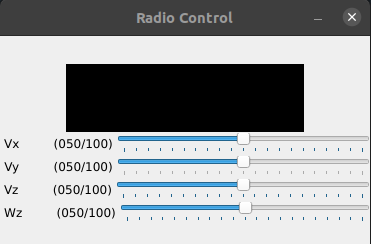
\includegraphics[height=4.5cm]{imagenes/cap4/2_axes_rc.png}
	\end{center}
	\caption[Primera versión del teleoperador]{Primera versión del teleoperador}
	\label{fig:teleoperador_v1}
\end{figure}

En el siguente paso, se buscó programar \textbf{comportamientos predefinidos}, es decir, acciones predeterminadas tales como desplazarse distancias concretas en ciertas direcciones, o girar un número específico de grados en un sentido u otro. Para ello, se diseñó una ampliación sobre la interfaz anterior, en la que se añadió un \textbf{botón por cada acción} concreta desarrollada, además de una \textbf{imagen de la cámara frontal} en directo. Es importante destacar la acción de moverse de distancias específicas, ya que se empleará en los algoritmos posteriores.\\

Finalmente, y continuando con lo anterior, se intentó afinar el comportamiento de las acciones predefinidas, para hacer que el dron se desplazase de celda en celda, concretamente de \textbf{centro en centro}. La idea es que, el dron solo tomará medidas de la señal en posiciones concretas y no en movimiento. Además, se agregaron \textbf{marcadores en \emph{rviz}}, para determinar las celdas visitadas (con colores aleatorios), junto con otro marcador que muestra la trayectoria que sigue la aeronave.\\

\begin{figure} [H]
	\begin{center}
	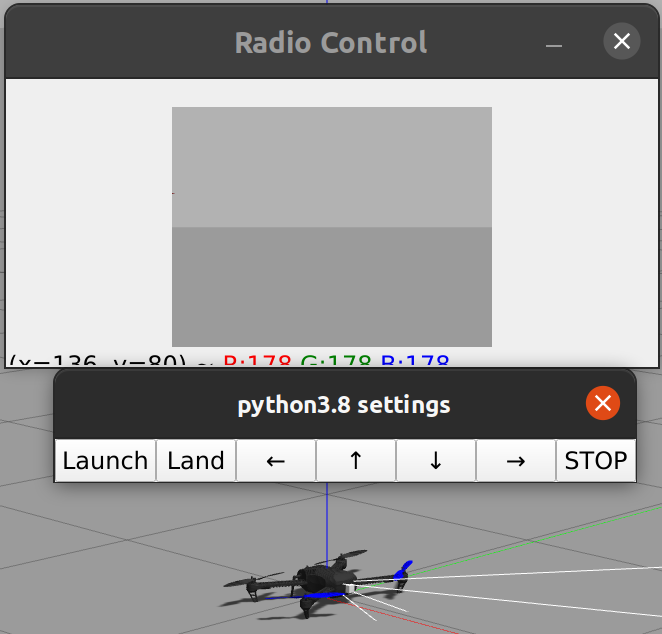
\includegraphics[height=8cm]{imagenes/cap4/3_c2c_gui.png}
	\end{center}
	\caption[Versión final del teleoperador]{Versión final del teleoperador}
	\label{fig:teleoperador_end}
\end{figure}

\newpage
A continuación, se muestra el \emph{``main''} de la aplicación mencionada:\\

\begin{code}[H]
\begin{lstlisting}[language=Python]
if __name__ == '__main__':
    try:
        rospy.init_node(NODENAME, anonymous=True)

        # Msgs
        ## Subscribers
        image_sub = rospy.Subscriber(IMAGE_TOPIC, Image, callback = image_cb)
        current_pos_sub = rospy.Subscriber(LOCAL_POSE_TOPIC, PoseStamped, callback = current_pos_cb)

        ## Publishers
        pos_pub = rospy.Publisher(RADIO_CONTROL_POS_TOPIC, PoseStamped, queue_size=10)
        cmd_pub = rospy.Publisher(RADIO_CONTROL_CMD_TOPIC, Px4Cmd, queue_size=10)

        # -- OPENCV -- #
        cv2.namedWindow(WINDOWNAME)

        # Buttons
        cv2.createButton('Launch', launch_button, None, cv2.QT_PUSH_BUTTON, 1)
        cv2.createButton('Land', land_button, None, cv2.QT_PUSH_BUTTON, 1)
        cv2.createButton('←', left_button, None, cv2.QT_PUSH_BUTTON, 1)
        cv2.createButton('↑', front_button, None, cv2.QT_PUSH_BUTTON, 1)
        cv2.createButton('↓', back_button, None, cv2.QT_PUSH_BUTTON, 1)
        cv2.createButton('→', right_button, None, cv2.QT_PUSH_BUTTON, 1)
        cv2.createButton('STOP', stop_button, None, cv2.QT_PUSH_BUTTON, 1)

        cv2.waitKey(0)
        cv2.destroyAllWindows()
    except rospy.ROSInterruptException:
        pass
\end{lstlisting}
\caption[Main de center to center app]{Main de center to center app}
\label{cod:c2c_app}
\end{code}

Donde, tras inicializar el nodo \ac{ROS}, se definen por un lado los \textbf{suscriptores}, encargados de recibir los datos de la cámara y la posición del dron (usando MAVROS), los \textbf{publicadores}, cuya función es enviar posiciones y/o comandos al script controlador, y por último la \textbf{interfaz gráfica} diseñada con \textbf{OpenCV}, donde se define la ventana y los botones con las diversas acciones predefinidas \footnote{Código completo en \url{https://github.com/RoboticsLabURJC/2022-tfg-cristian-sanchez/blob/main/src/teleop/scripts/c2c_control.py}}.\\

\section{Señales}
\label{sec:signals}

Continuando con el proyecto, entramos en el segundo gran bloque, las \textbf{señales \ac{RF}}. Este apartado fue especialmente relevante, ya que nos permitió desarrollar una aplicación reactiva, con la meta de generar entornos sobre los que probar soluciones robóticas.\\

Pero, antes de entrar en detalle en estos aspectos, conviene familiarizarse con algunos \textbf{conceptos básicos} sobre el \textbf{procesamiento de señales}:

\begin{enumerate}
	\item \emph{Señal}: se trata de una función que describe un fenómeno físico, y que se emplea para la transmisión de información.

    \item \emph{Dominio temporal}: establece el eje de abcisas con el tiempo.

    \item \emph{Dominio de la señal}: determina si la señal se expresa en tiempo o en frecuencia (a través de transformadas).

    \item \ac{ADC}: elemento electrónico que permite la conversión de señales analógicas a señales digitales.

    \item \ac{RSSI}: permite establecer el nivel de potencia de una señal, con respecto a 1 mW de potencia. Se expresa en dBm.

    \item \ac{SNR}: métrica que permite medir la potencia de la señal con respecto al ruido ambiente.

    \item \emph{Frecuencia}: parámetro de la función que define a la señal, el cual determina el número de veces que se repite en un segundo. Se mide en hercios (Hz).

    \item \emph{TX}: Se refiere a la transmisión de la señal.

    \item \emph{RX}: Hace referencia a la recepción de la señal.
\end{enumerate} \cite{basics-signals}\\

Definidos estos términos, nuestro objetivo se basó en obtener un modelo capaz de calcular la \textbf{propagación de la señal}, es decir, un sistema capaz de calcular como se comporta la potencia de una señal, según las características de su entorno.\\

\subsection{Aproximación de Friis}
\label{subsec:friis}

Por ello, se optó por emplear la aproximación de Friis, que nos proporciona una sencilla fórmula sobre la cual modelizar nuestro problema:

\begin{align}
    P_r = P_t \cdot \left( \frac{G_t G_r \lambda^2 }{(4 \pi)^2 d^n L} \right)
\end{align}

Donde cada término significa lo siguiente:

\begin{enumerate}
    \item \emph{$P_t$ y $P_r$}: aluden a la potencia del transmisor y la potencia del receptor respectivamente.

    \item \emph{Ganancias} ($G_t$, $G_r$): representan un valor incremental aplicado a la potencia de emisión y de recepción, respectivamente.

    \item \emph{Valor lambda} ($\lambda$): hace referencia a la longitud de onda. Está directamente relacionado con la frecuencia.

    \item \emph{Distancia} (d): desde el origen de la señal a un punto en el espacio.

    \item \emph{L}: representa todas aquellas pérdidas no asociadas a la propagación de la señal.

    \item \ac{PLE} (n): permite ajustar el modelo a diversos entornos. Es un valor constante extraido de forma empírica. A continuación se muestra una tabla con varios ejemplos.
\end{enumerate} \cite{friis-1}\\

\begin{figure} [H]
	\begin{center}
	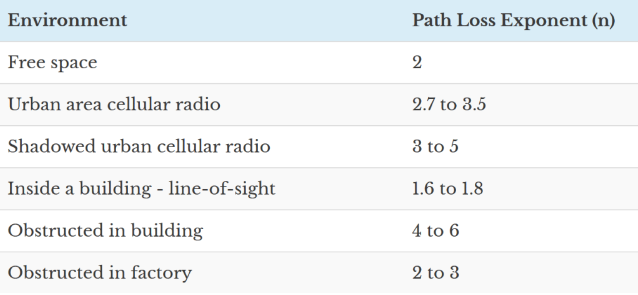
\includegraphics[height=5cm]{imagenes/cap4/4_PLE_table.png}
	\end{center}
	\caption[Tabla ejemplos exponente n]{Tabla ejemplos exponente n}
	\label{fig:ple_table}
\end{figure}

Además, empleando este método, podemos modelizar las \textbf{pérdidas de una señal} estimadas durante su propagación, a través de la siguiente ecuación:\\

\begin{align}
    P_L(dB) = -10 \log_{10} \frac{\lambda^2}{(4 \pi d)^2}
\end{align}

Sin embargo, para nuestro caso no es relevante (aunque está incluido dentro del módulo).\\

\subsection{Módulo python de Friis}
\label{subsec:friis-module}

Una vez realizadas las pruebas iniciales, se buscó compactar todo, de forma que fuera accesible para cada aplicación que lo necesitase.\\

Por ello, surgió la idea de crear un \textbf{módulo python} que se encargará de modelizar las ecuaciones previamente mencionadas. Para ello, se diseño una clase cuyo constructor se encargara de recibir, por parámetros, las variables implicadas en las ecuaciones de Friis, además de las dimensiones del mapa y su resolución (la cual afecta al tamaño de celda).\\

Básicamente, el \textbf{proceso} seguido para usar este módulo es el siguiente, primero se crea un objeto de la clase Friis donde se especifican las características de la señal y las variables relacionadas con el mapa, lo que genera internamente un array 2D vacío, que será rellenado en función del modelo seleccionado. Posteriormente, se selecciona el modelo deseado (propagación o pérdidas, este último no está testeado), pasando las coordenadas del origen de la señal por parámetros. Esto, retornará el mapa relleno con los valores asociados a las ecuaciones del modelo de Friis seleccionado.\\

A continuación se mostrará un ejemplo sencillo de uso, donde se obtendrá un mapa de propagación de señal, en forma de Numpy array 2D:

\begin{code}[H]
    \begin{lstlisting}[language=Python]

    #! /usr/bin/env python
    import friss as fr

    if __name__ == '__main__':
        friis_object = fr.Friss(power_tras=10.0,
                                gain_tras=1.5,
                                gain_recv=2.0,
                                freq=fr.FREQ_WIFI,
                                losses_factor=1.0,
                                losses_path=2.0,
                                world_sz=(10,10),
                                resolution=1.0)

        signal_map = friis_object.model_power_signal(origin=(5,3))

\end{lstlisting}
\caption[Ejemplo básico de uso del módulo Friis]{Ejemplo básico de uso del módulo Friis}
\label{cod:friis_basics}
\end{code}

Yendo al detalle, se puede ver que se genera un mapa 10x10 con resolución 1 (es decir, cada celdilla es de 1x1 unidades), de una señal WIFI, donde el transmisor emite a 10 W, con una ganancia de 1.5, el receptor posee una ganancia de 2, un factor de pérdidas (L) de 1, es decir, sin pérdidas, y por último, el exponente n (\ac{PLE}) con un valor de 2, que representa el espacio vacío. Luego se genera el mapa de propagación de la señal, indicando que la fuente se encuentra en las coordenadas (5,3).\\

No obstante, este módulo posee \textbf{otras funcionalidades} útiles para trabajar con él, como son:

\begin{enumerate}
    \item \textbf{\emph{reset\_world}}: modifica el mapa que hubiera, estableciendo todos sus valores a cero.

    \item \textbf{\emph{get\_world\_sz}}: retorna las dimensiones del mapa.

    \item \textbf{\emph{set\_values}}: modifica las características de la señal simulada.
\end{enumerate}

Hay que tener en cuenta que, aunque se modifiquen los parámetros, se debe modelar de nuevo el mapa para que surtan efectos los cambios.\\
\newpage
Por último, se busco \textbf{extender la funcionalidad del módulo}, de manera que fuera posible incluir obstáculos en el mapa. La idea era crear un método capaz de posicionar \textbf{obstáculos} en el mapa de la señal, y simular su efecto en la señal.\\

Para ello, se buscó trazar proyecciones desde la señal hasta los bordes del obstáculo, de forma que se generase un polígono con los bordes del mapa. Posteriormente, se revisó que puntos se encontraban dentro del polígono (que no fueran propiamente parte del obstáculo), a través de un algoritmo basado en el número de intersecciones del punto con el perímetro del polígono, trazando una línea horizontal y hacia la derecha \cite{poly-info}. Por último, para cada punto dentro del polígono se le aplicó un factor de pérdida al valor almacenado de la señal, de manera que se simulase el efecto del obstáculo.\\

\begin{figure} [H]
	\begin{center}
	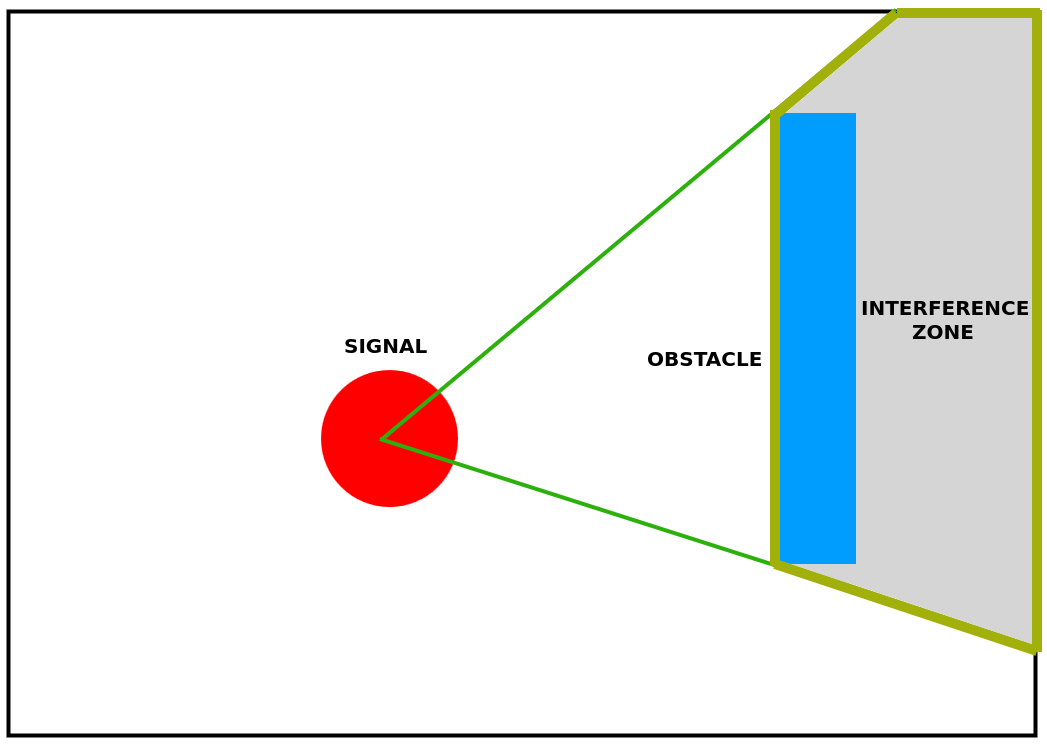
\includegraphics[height=7cm]{imagenes/cap4/5_interference.png}
	\end{center}
	\caption[Representación del algoritmo]{Representación del algoritmo}
	\label{fig:interference_algorithm}
\end{figure}

La idea fue abrir puertas a nuevos entornos más complejos y realistas, sobre los que poder probar diversas soluciones, en nuestro caso, para testear el efecto de un muro en el camino del dron a la señal.\\
\newpage
\subsection{Aplicación de Friis}
\label{subsec:friis-app}

La última sección relacionada con las señales se centro en integrar el módulo previo, en una \textbf{interfaz gráfica intuitiva para el usuario}. La idea era estudiar, en tiempo real, como evolucionaba la señal cuando alguno de sus parametros, en la ecuación de Friis, era modificado.\\

Para llevarlo a cabo, se empleó la librería \textbf{matplotlib}, debido a la enorme cantidad de herramientas de las que dispone, así como de su sencillez a la hora de crear nuevas aplicaciones. Funciona de manera que se generan eventos que son gestionados en \emph{``callbacks''}, es decir, se generan bucles asociados a dichos eventos, que reaccionan a cambios en la interfaz generada.\\

En nuestro caso, la \textbf{estructura base} consta de una figura, sobre la que se agregan todos los elementos, entre los que encontramos los mapas de calor o \emph{``heatmap''} en forma de plots, las barras de acción o \emph{``sliders''}, botones, entre otros elementos que se explicarán más adelante.\\

Inicialmente, se optó por representar un mapa de calor con una barra de color asociada a los distintos valores de la señal. Además, se integraron sliders correspondientes a cada valor presente en la ecuación de Friis, tal y como se muestra a continuación:\\

\begin{figure} [H]
	\begin{center}
	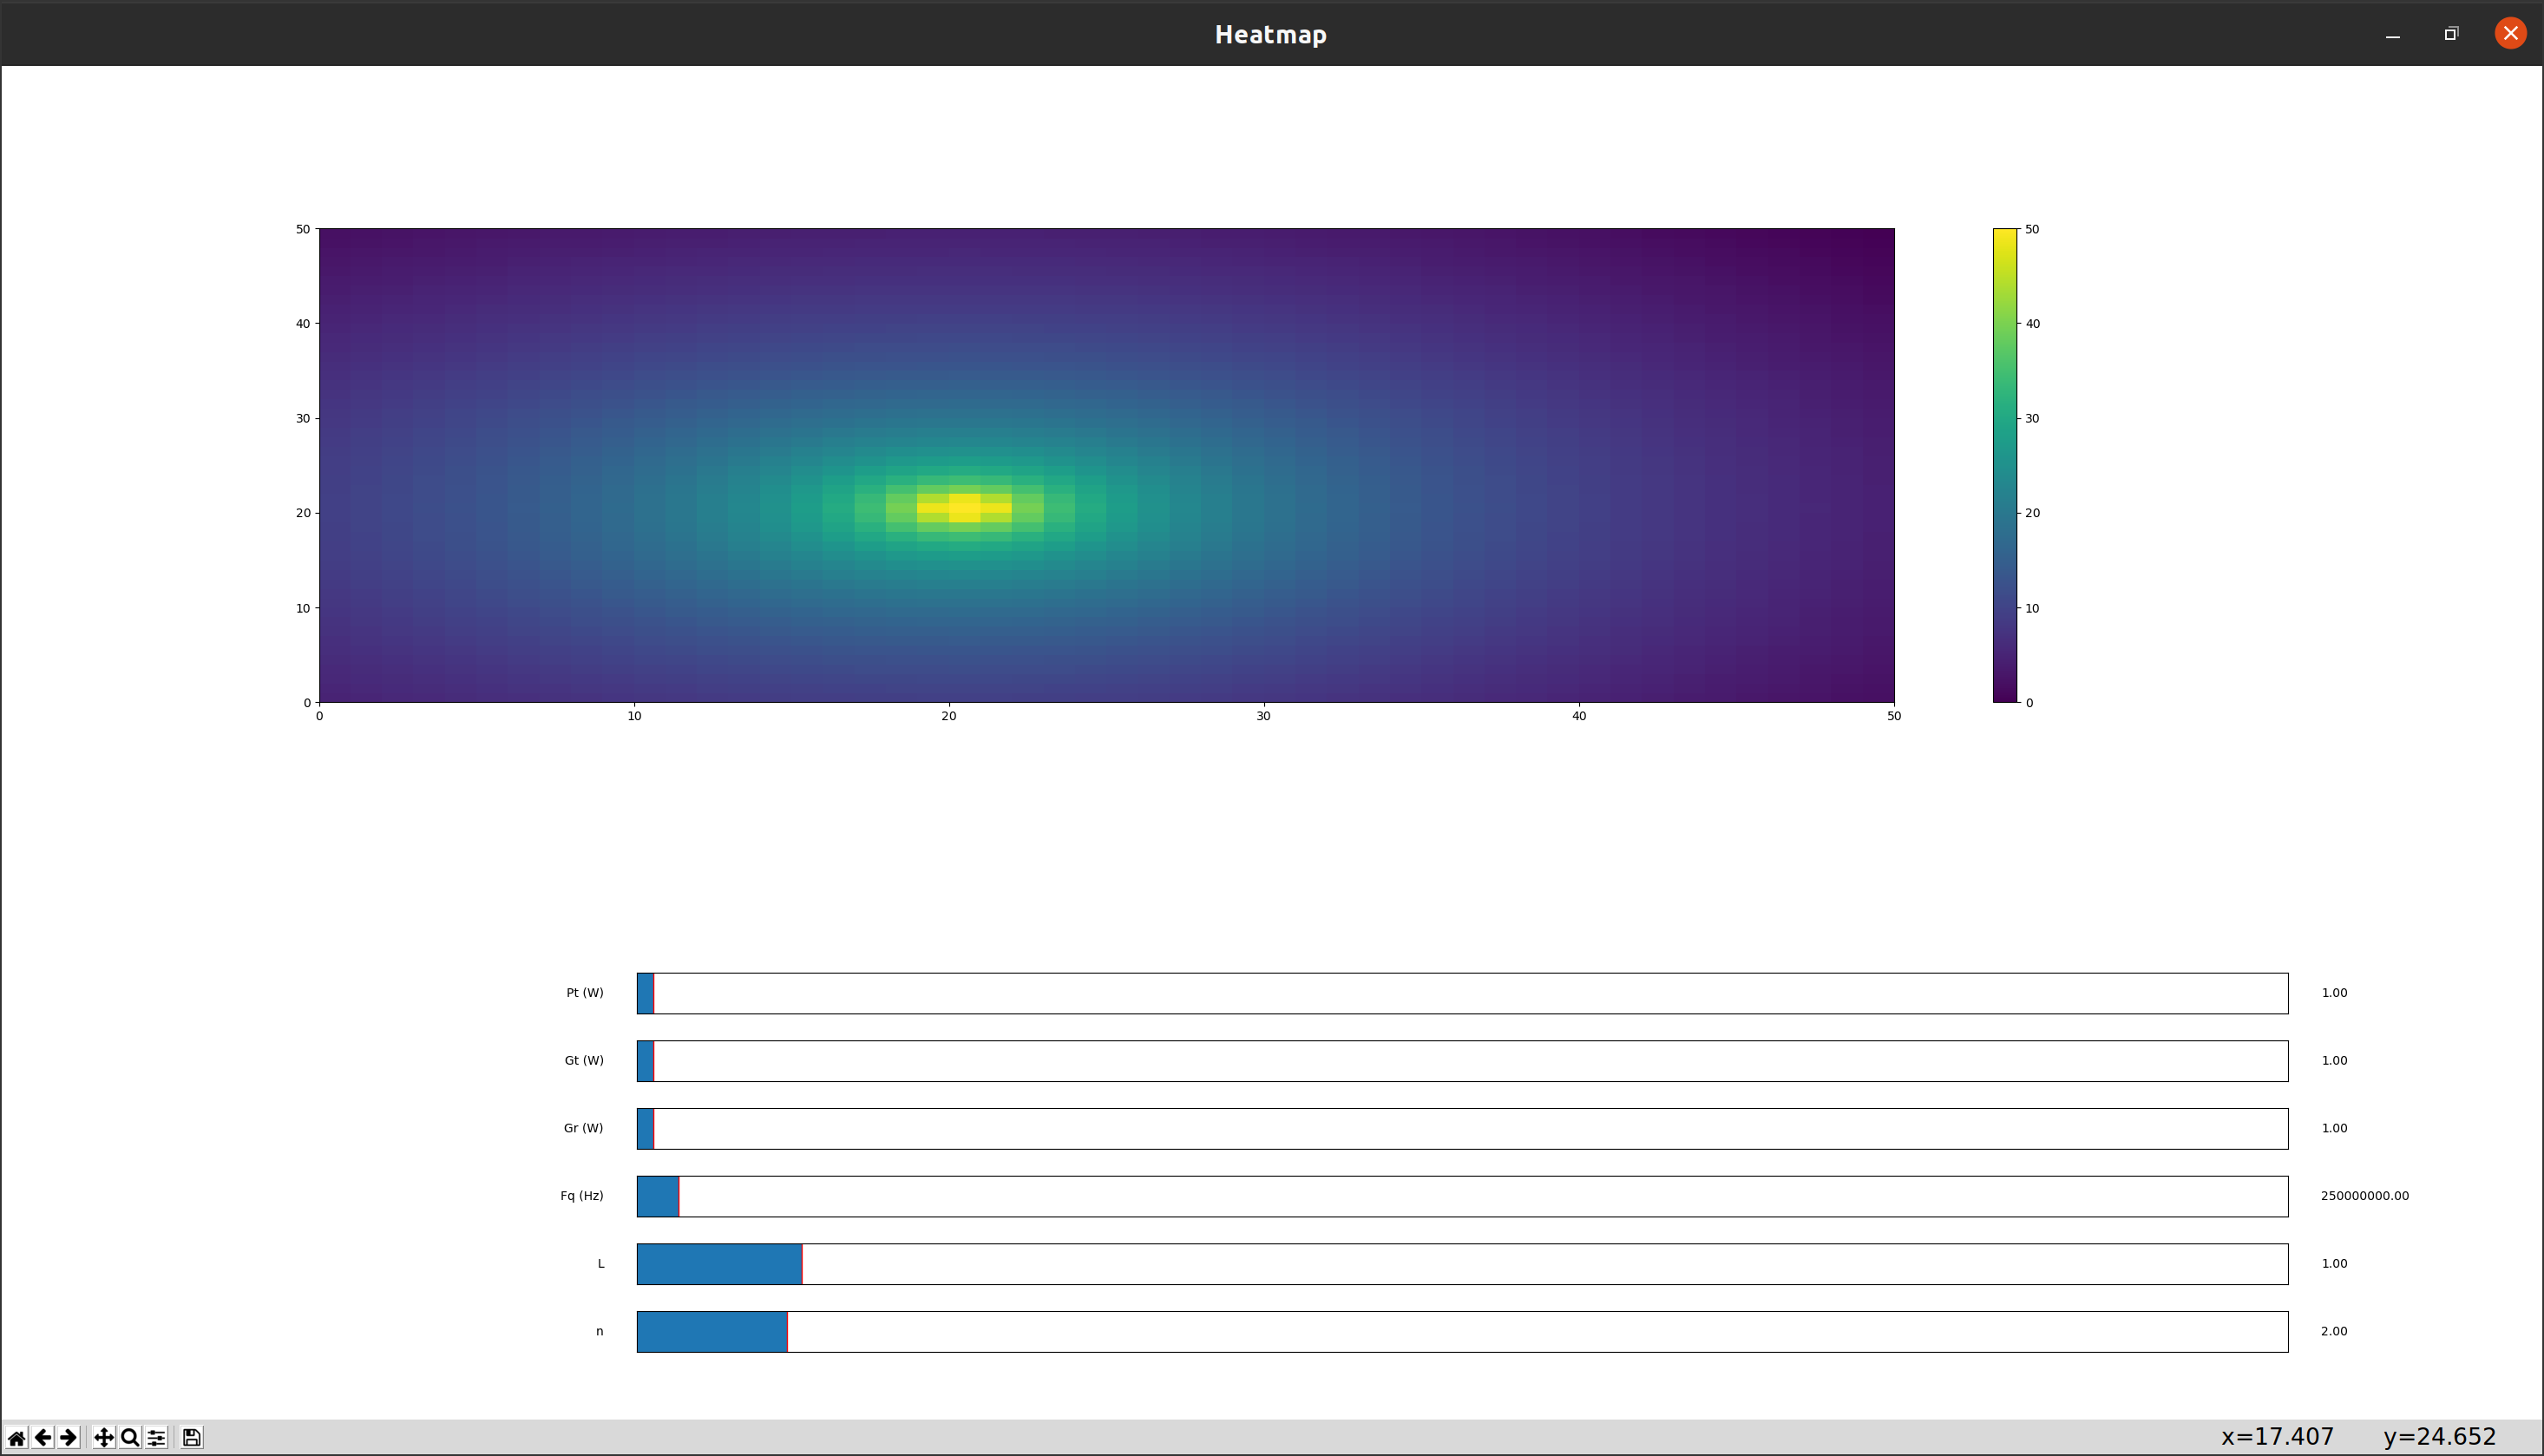
\includegraphics[height=7cm]{imagenes/cap4/6_Friss_firstGUI.png}
	\end{center}
	\caption[Primera versión de la interfaz]{Primera versión de la interfaz}
	\label{fig:friis_init_app}
\end{figure}
\newpage
El problema fue, que al actualizar los valores, también lo hacía la representación, por lo que no se apreciaba el efecto de los cambios en el plot.\\

Por ello, se agregaron dos mapas de calor, uno con el máximo y el mínimo fijados a mano (donde sí se aprecian los cambios), y el anterior mencionado. Para elegir cual usar, se agregó una casilla marcable. Además, se incluyeron dos variables relevantes a la hora de modelar, el \textbf{tamaño del mapa} y la \textbf{resolución}, manejadas a través de \emph{``sliders''}, los cuales a su vez se activan al pulsar un botón de \textbf{SET}, que recarga la interfaz. Además, se ajustó los saltos de valores para que fueran coherentes en el resto de barras de acción, tal y como se puede apreciar a continuación:\\

\begin{figure} [H]
    \begin{center}
    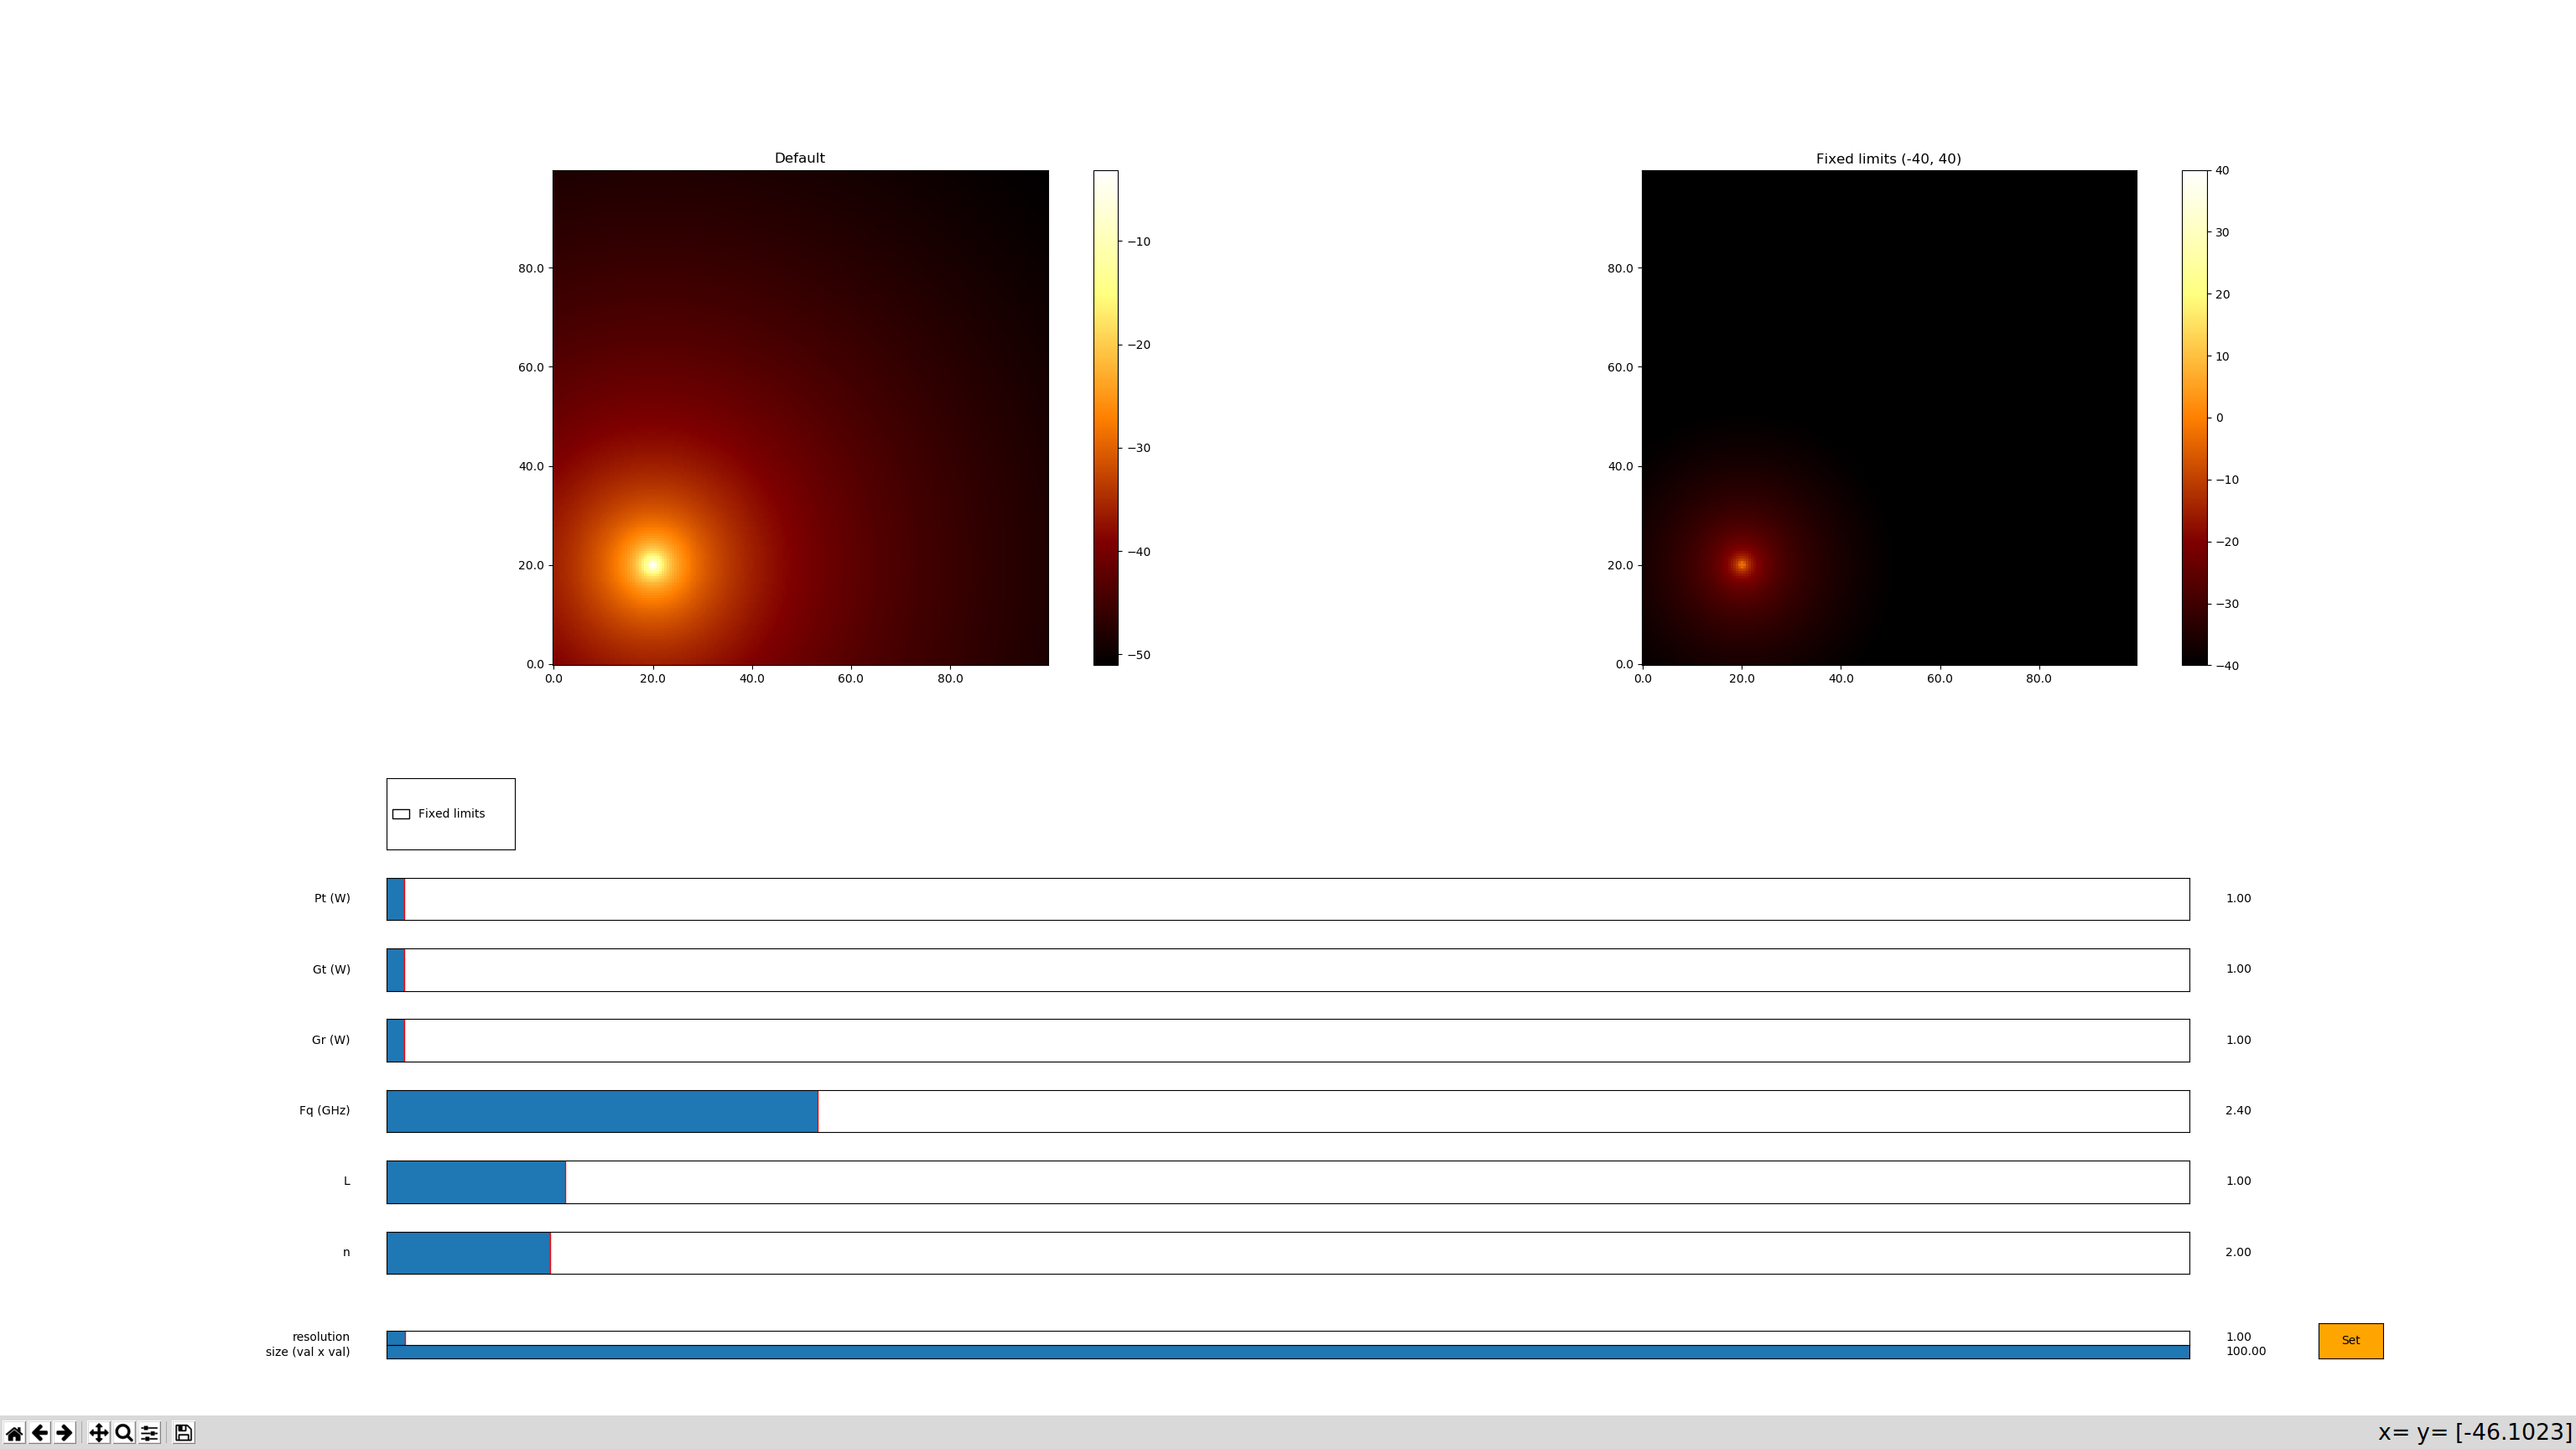
\includegraphics[height=8cm]{imagenes/cap4/7_Friss_endGUI.png}
    \end{center}
	\caption[Versión final de la interfaz]{Versión final de la interfaz}
	\label{fig:friis_end_app}
\end{figure}

Cabe destacar que, por motivos de desarrollo, no se agregó la parte de generación dinámica de obstáculos a la aplicación, ya que esta se desarrollo como un extra al final del \ac{TFG}.\\

\newpage
\section{Integración conjunta}
\label{sec:integration}

La integración conjunta engloba la parte final del proyecto, es la fase donde se juntaron las secciones anteriores, con el fin de generar el entorno deseado para resolver el problema.\\

El objetivo, a parte de llevar a cabo la tarea encomendada, era comprobar y comparar los distintos algoritmos entre sí, a través de diversas métricas de rendimiento.\\

\subsection{Primeros pasos}
\label{subsec:primeros_pasos}

Inicialmente, se debía construir todo el entorno en base a lo anterior.\\

Por ello, se diseñó una \textbf{aplicación servidor de datos}, que funciona como intermediaria con el módulo de Friis. Siendo concisos, dicha aplicación contiene \textbf{dos servidores} basados en \textbf{acciones \ac{ROS}}, que son especialmente útiles en este caso, dada su naturaleza asíncrona. Dichos servidores gestionan las peticiones para el dron y para rviz. A continuación detallamos cada caso:

\begin{enumerate}
	\item \emph{Caso dron}: a groso modo, el dron envía su posición en coordenadas transformadas al sistema de referencia del \emph{``heatmap''}, y recibe el valor de la señal de dichas coordenadas. En un caso real, el dron tan solo accedería al valor de la señal a través de un sensor que se lo permitiera. A posteriori, se agregó la funcionalidad de enviar, en dicha petición, si se deseaba un mapa con obstáculos o no.

	\item \emph{Caso rviz}: recibe una petición donde se agregan todas las características de la señal para generar el \emph{``heatmap''} deseado, vease el origen y sus componentes. Esto, genera como respuesta un array de floats que contiene la información del mapa de calor, en un formato adecuado para su representación, es decir, para generar el mapa de forma gráfica, se emplea la biblioteca \textbf{grid\_map}, que a través de un topic de \ac{ROS}, permite enviar los datos a un plugin de rviz, el cual genera la representación visual buscada\footnote[2]{Toda la funcionalidad englobada en el directorio \textbf{heatmap\_util} del proyecto}. También se agregó la funcionalidad de los obstáculos para experimentación futura.
\end{enumerate}
\newpage
\subsection{Algoritmos}
\label{subsec:algoritmos}

En esta sección, se resume el núcleo del proyecto. Es el lugar donde se mostrarán todas las soluciones implementadas para comandar al dron hacía la resolución del problema y se explicará, desde la estructura general de la aplicación, hasta la lógica empleada detrás de cada algoritmo.\\

Por ello, lo primero consistió en definir una \textbf{clase \emph{``Drone''}}, cuyo constructor se encargara de conectar los topics al controlador PX4 para comandar ordenes a la aeronave. Además, establece la comunicación con el servidor de datos (tanto para la potencia como para rviz) y se definen los diferentes atributos pertenecientes a la clase, que en este caso aluden a parámetros necesarios para los algoritmos y la extracción de resultados.\\

En general, la clase sigue una estructura basada en lo siguiente:

\begin{enumerate}
	\item \emph{Métodos para comandar al dron}: o conjunto de funciones encargadas del movimiento del dispositivo (como despegar, aterrizar, desplazarse, entre otros). Mucha de esa funcionalidad fue adaptada del teleoperador realizado al inicio del \ac{TFG}.

    \item \emph{Métodos de tolerancia}: encargados de establecer un margen aceptable entre la posición del dron y el objetivo deseado. Estos métodos sirven para controlar con precisión problemas que surgen de la deriva y de condiciones externas, como puede ser el viento.

	\item \emph{Métodos de conversión}: que en este caso nos permiten transformar las coordenadas entre los sistemas de referencia, tal y como se puede apreciar a continuación.

    \item \emph{Algoritmos}: o las soluciones propiamente dichas, que en sí contienen el conjunto de métodos que cada cual necesita para llevarse a cabo. Podemos distinguir entre \textbf{manual, manual optimizado y Q-Learning}.
\end{enumerate}

\begin{figure} [H]
    \begin{center}
    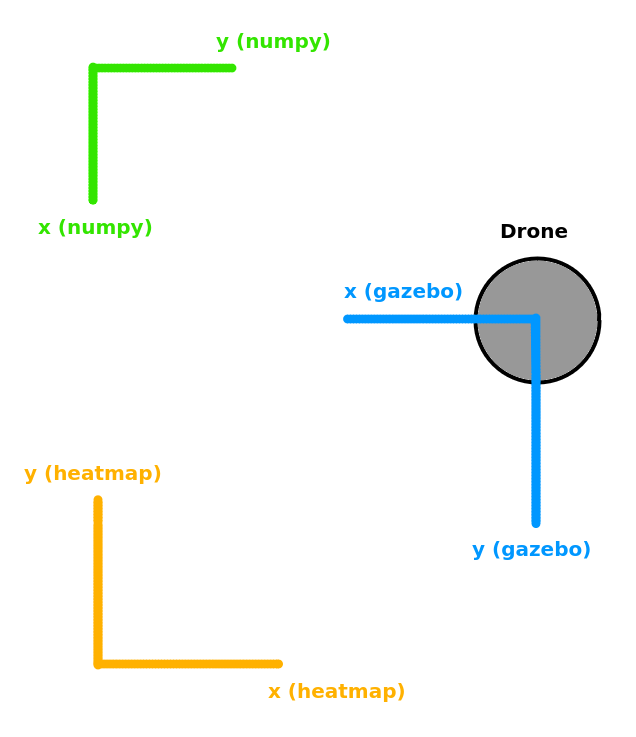
\includegraphics[height=10cm]{imagenes/cap4/8_reference_system.png}
    \end{center}
    \caption[Sistemas de referencia]{Sistemas de referencia}
    \label{fig:reference_sys}
\end{figure}

En cuanto al desarrollo propiamente dicho de los algoritmos, se deben cumplir una serie de premisas de cara a la simulación.\\ 

Primero que, \textbf{todos los movimientos realizados por el dron deben estar contenidos en el mapa de calor generado}; además, \textbf{la medida de la señal} sólo podrá tomarse cuando el dron esté en el \textbf{centro de la celda}; los movimientos del dron deberán ser \textbf{de centro en centro} aunque esto abarque más celdas de distancia (problema resuelto y adaptado del teleoperador); y cada celda mide 1x1 metros.

\subsubsection{Algoritmo manual}
\label{subsec:alg-manual}

Es básicamente la primera aproximación, consiste en \textbf{visitar todos los vecinos más cercanos} y realizar el desplazamiento hacia las coordenadas del \textbf{vecino con mayor señal} medida.\\

La \textbf{condición de parada} se basa en analizar si, las coordenadas objetivo de la iteración anterior son las mismas que las coordenadas objetivo de la iteración actual, además de que se cumpla que todos los vecinos colindantes tengan menor valor de señal mencionado.\\

En cuanto a los métodos que usa, se encuentra el de verificar movimientos válidos y comprobar si ha llegado al final, mediante la verificación de que todos los vecinos adyacentes, tienen potencias de señal inferior.\\

\begin{figure} [H]
    \begin{center}
    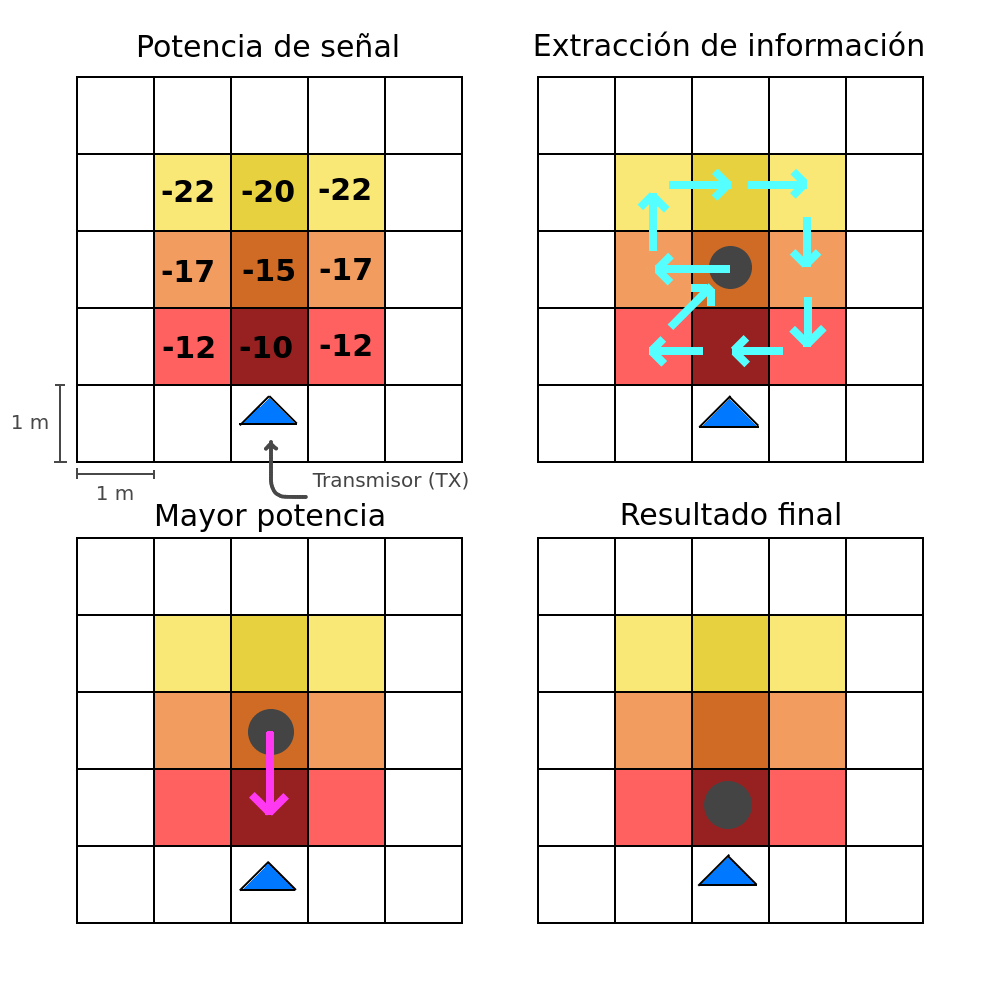
\includegraphics[height=10cm]{imagenes/cap4/9_algoritmo_manual.png}
    \end{center}
    \caption[Representación algoritmo manual]{Representación algoritmo manual}
    \label{fig:manual_algorithm}
\end{figure}

\subsubsection{Algoritmo manual (optimizado)}
\label{subsec:alg-manual-opt}

Tomando como referencia el algoritmo anterior, se buscó agregar ciertas mejoras y eficiencia. El principio es el mismo, obtener la información de los vecinos y navegar hacia el mejor candidato.\\

La diferencia radica en \textbf{no revisitar vecinos} cuya información se conozca. Para ello se implementa un array que almacena hasta 18 coordenadas de vecinos visitados, de modo que solo se navega hacia coordenadas no contenidas en el mismo, y que por supuesto cumplan las condiciones del problema (no salir del mapa de calor, mover de centro a centro, entre otras).\\

La condición de parada es idéntica a la anterior, y los métodos usados también.\\

\begin{figure} [H]
    \begin{center}
    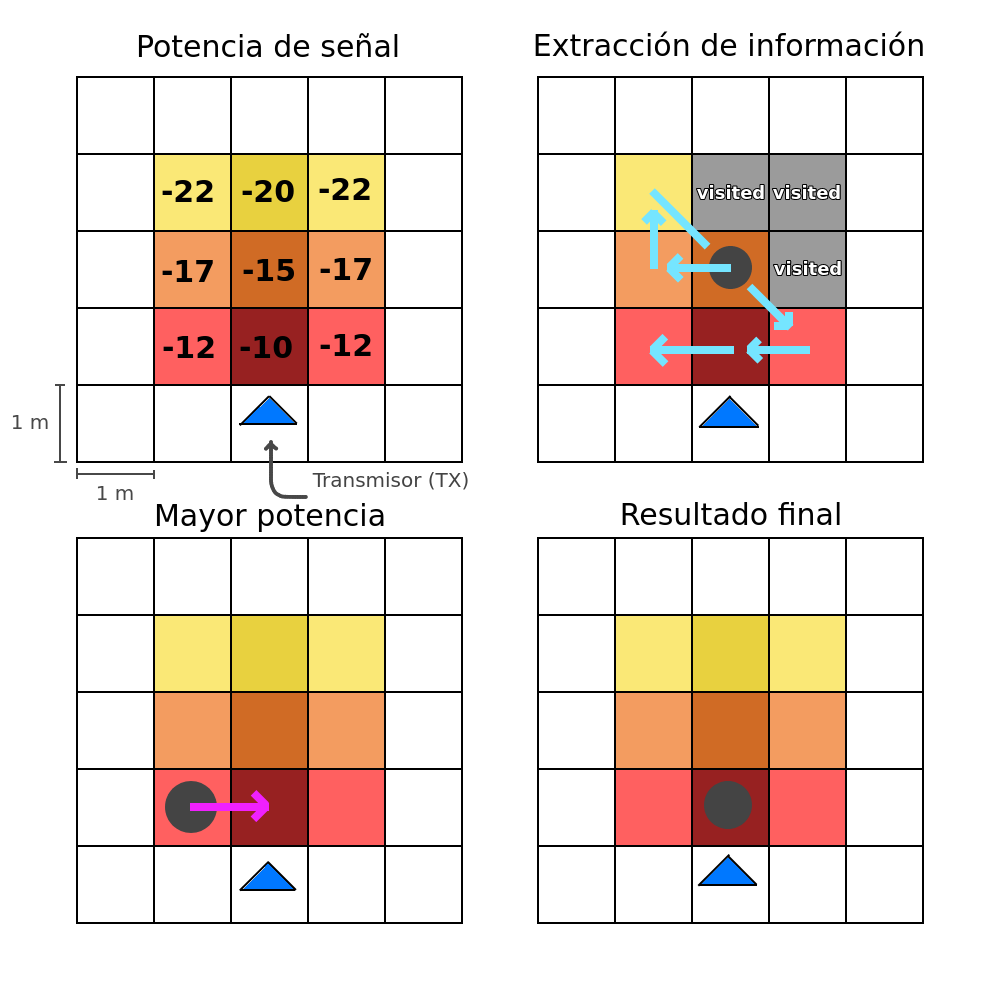
\includegraphics[height=10cm]{imagenes/cap4/10_algoritmo_optimizado.png}
    \end{center}
    \caption[Representación algoritmo manual optimizado]{Representación algoritmo manual optimizado}
    \label{fig:opt_algorithm}
\end{figure}

\subsubsection{Algoritmo Q-Learning}
\label{subsec:alg-q}

El último algoritmo planteado, se basó en técnicas de \textbf{aprendizaje por refuerzo}. Concretamente empleando Q-Learning, que tal y como comentamos al principio de la memoria, consiste en la obtención de una tabla Q, de estados y acciones, donde se asignan valores numéricos cada acción según su estado, de modo que la acción más favorable acaba teniendo mayor valor que el resto.\\

En nuestro caso, los \textbf{estados} son \textbf{las coordenadas del dron} en términos del mapa de calor, y las \textbf{acciones} son los \textbf{movimientos cardinales y diagonales}, de una o más celdas de distancia.\\

Como todo algoritmo de esta naturaleza, posee dos fases bien diferenciadas, la \textbf{fase de entrenamiento}, cuyo objetivo es rellenar de forma eficaz la tabla Q, y la \textbf{fase de inferencia}, donde se prueban los resultados obtenidos del entrenamiento.\\

Dentro del entrenamiento, distinguimos los \textbf{episodios}, que en nuestro caso son las llegadas a la fuente, o las salidas del mapa de calor (adicionalmente se probó añadir otra condición que fuera basada en el número de malas acciones consecutivas, pero para nuestra solución se decidió obviar); y las \textbf{iteraciones}, que se definen como el desempeño de una acción literalmente.\\

Además, para rellenar el contenido de la tabla, se definieron las pertinentes \textbf{recompensas y penalizaciones} basadas en la diferencia entre la medidas, antes y después de realizar una acción (agregando un pequeño multiplicador a las recompensas negativas), excepto si se sale del mapa, en cuyo caso se establece una recompensa fija negativa, calculada en proporción al resto de recompensas. Posteriormente se asignan valores en la tabla Q, usando la ecuación de Bellman:
\begin{equation}
    Q(s, a) = (1 - \alpha) \cdot Q(s, a) + \alpha \cdot \left(r + \gamma \cdot \mathrm{max}_{a'} Q(s', a')\right)
\end{equation}
Cabe destacar que, durante el entrenamiento, se especifican una serie de parámetros que fueron ajustados a través de la experimentación, entre los que se encuentran: el \textbf{número de episodios totales}, que repercute directamente en la \emph{fase de exploración} (detallado a continuación); el \textbf{parámetro $\alpha$}, o la tasa de aprendizaje, que afecta a la convergencia de las soluciones durante el aprendizaje; el \textbf{parámetro $\gamma$}, o factor de descuento, que atañe a la importancia de las acciones futuras con respecto a las inmediatas; y por último los valores de \textbf{epsilon ($\epsilon$)}, que determinan si la acción tomada será aleatoria o extraida de la tabla, esto está directamente asociado a la \emph{fase de exploración}, donde se prioriza la aleatoreidad con el fin de enriquecer con información la tabla Q.\\

En nuestro caso, esta fase ocupa un \textbf{20\% del número de episodios}, de forma lineal, es decir, que cada vez la prioridad se va decantando más del lado de la tabla y no de la aleatoreidad (durante el entrenamiento siempre se mantiene cierta posibilidad de tomar una acción arbitraria, para seguir actualizando los datos).\\

Para poder entrenar de forma eficiente, se establecieron distintos puntos de entrenamiento repartidos de forma uniforme por el mapa, hablaremos en detalle de esto, en la sección de métricas empleadas.\\

Los métodos usados para Q-Learning, se basan en funcionalidades necesarias para desempeñar todo lo anterior, véase la generación de estados y acciones para la tabla, la extracción de índices dentro de la misma, el tratamiento del parámetro $\epsilon$, la obtención de coordenadas válidas, entre otros\footnote[3]{Todos los métodos están explicados dentro del código \url{https://github.com/RoboticsLabURJC/2022-tfg-cristian-sanchez/blob/main/src/teleop/scripts/algorithms.py}}.\\

\begin{figure} [H]
    \begin{center}
    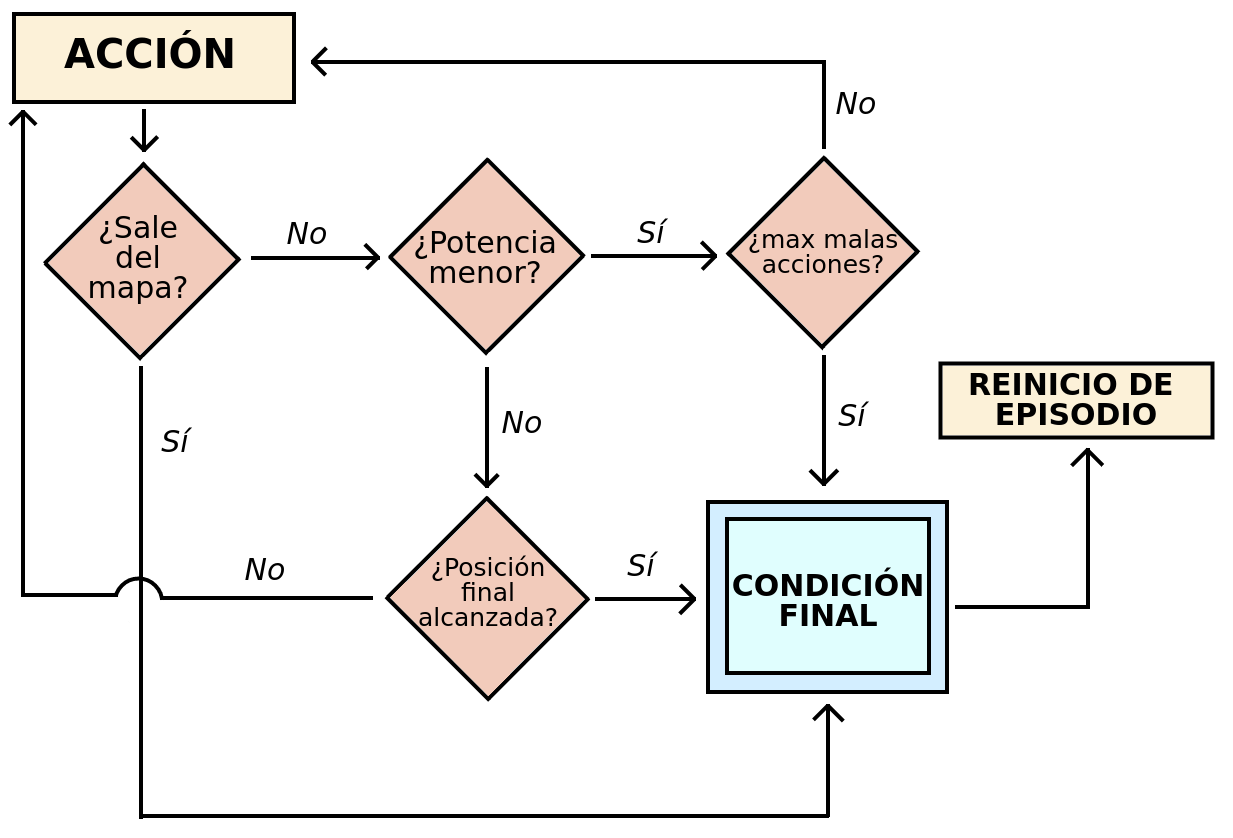
\includegraphics[height=10cm]{imagenes/cap4/11_diagrama_training.png}
    \end{center}
    \caption[Esquema episodio fase de entrenamiento]{Esquema episodio fase de entrenamiento}
    \label{fig:training_phase}
\end{figure}

Cabe resaltar que, si la acción tomada lleva al dron hacia una condición de final, este acaba el episodio, viaja hacia una nueva posición de entrenamiento y actualiza ciertos parámetros, como por ejemplo el parámetro $\epsilon$. La condición de final se aplica siempre tras actualizar los valores.\\

Por último, en la \emph{fase de inferencia}, el dron analiza su estado (o sus coordenadas dentro del mapa de calor), y observa la mejor acción disponible dentro de la tabla Q ya rellena. Esto lo realiza hasta que detecta la condición de parada, que se cumple cuando la medida anterior de señal es mayor que la actual y todos los vecinos adyacentes a la medida anterior poseen señal inferior. Para hacer un correcto análisis, se parte siempre de coordenadas distintas a las que se usaron para entrenar y rellenar la tabla Q.\\
\newpage
\subsection{Métricas empleadas}
\label{subsec:metricas}

He decidido comentar las métricas empleadas en una sección individual, debido a la importancia que poseen de cara al desarrollo y los resultados del proyecto.\\

En primer lugar se encuentra el \textbf{mapa de puntos}. Aquí se muestran las posiciones en el mapa de calor donde el dron entrenará, hará la inferencia (o desde donde partirá en los algoritmos manuales), además de la posición de la señal y propios los límites del mapa.\\

\begin{figure} [H]
    \begin{center}
    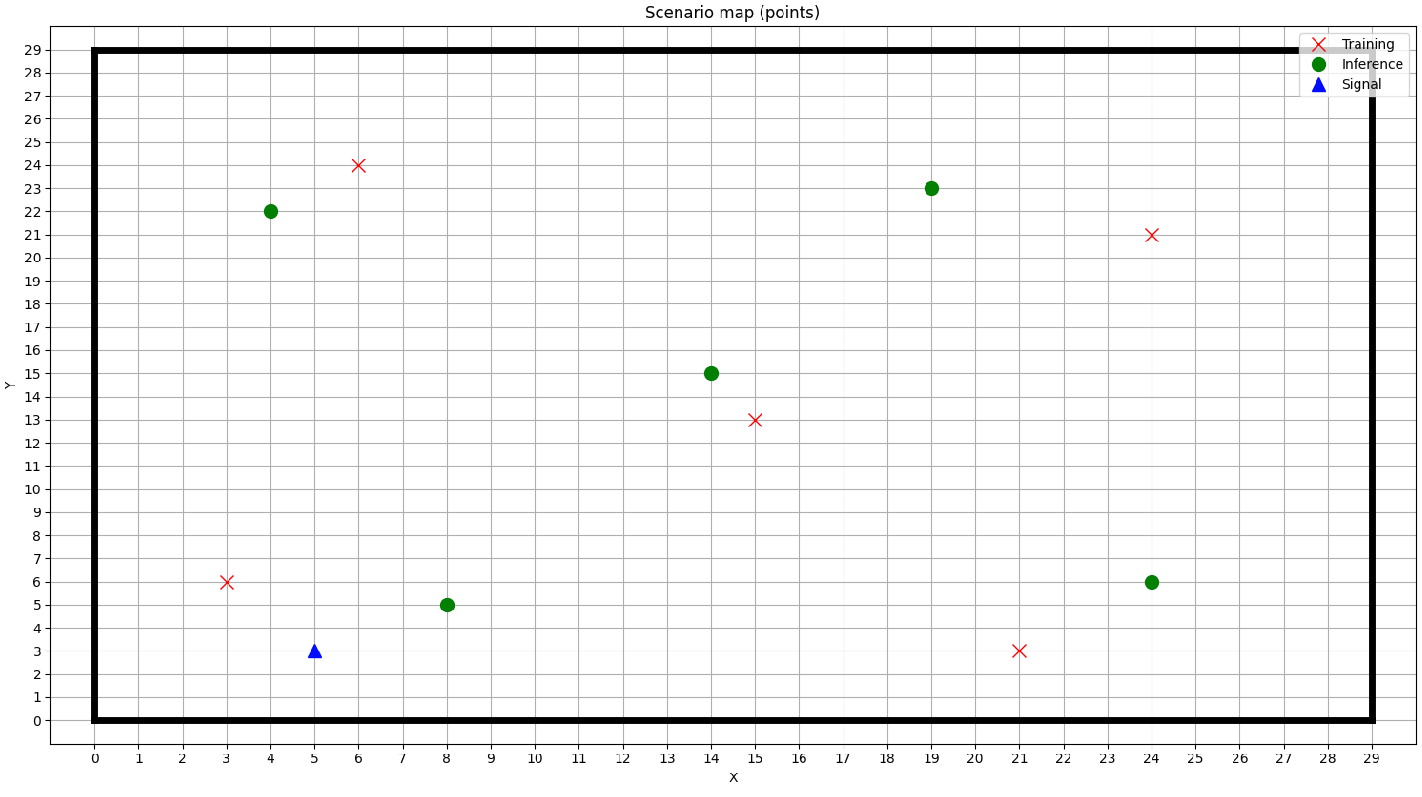
\includegraphics[height=7cm]{imagenes/cap4/12_puntos_30_esquina.png}
    \end{center}
    \caption[Mapa de puntos 30x30 con la señal en la esquina]{Mapa de puntos 30x30 con la señal en la esquina}
    \label{fig:30_points}
\end{figure}

El siguiente gráfico representa el \textbf{camino seguido} por el dron al aplicar cada algoritmo para unas mismas coordenadas.\\

\begin{figure} [H]
    \begin{center}
    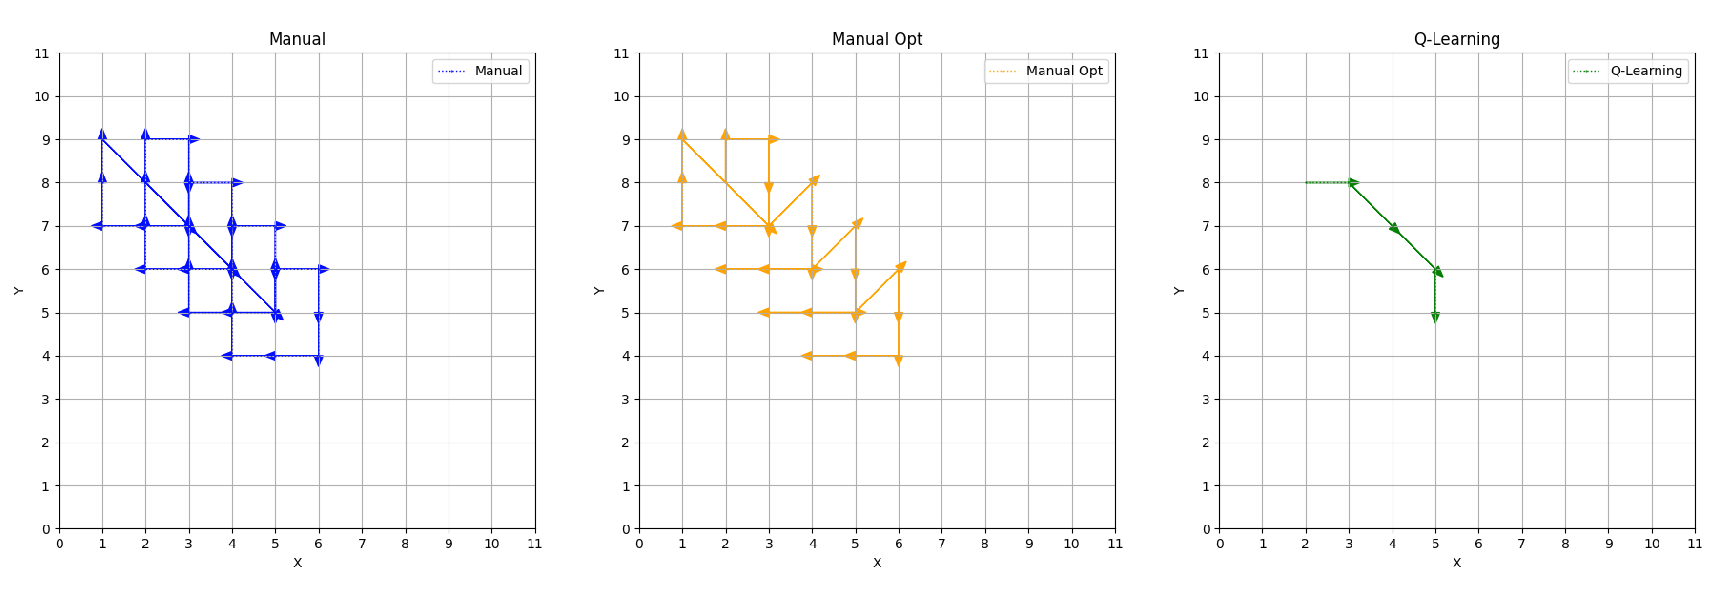
\includegraphics[height=5cm]{imagenes/cap4/13_trayectorias_12.png}
    \end{center}
    \caption[Trayectorias seguidas en mapa 12x12 con señal en el centro]{Trayectorias seguidas en mapa 12x12 con señal en el centro}
    \label{fig:12_traj}
\end{figure}

A continuación se presenta uno de los gráficos más relevantes, en este caso, un gráfico triple que nos permite \textbf{conocer en detalle como ha ido el entrenamiento}. En concreto, representa tres métricas: el valor de \textbf{epsilon} ($\epsilon$), en el que se distingue la fase de exploración; la \textbf{recompensa acumulada}, que nos permite analizar la convergencia del entrenamiento; y el \textbf{número de iteraciones}, donde se observa que conforme el algoritmo aprende, el número se reduce. Todo ello con respecto a cada episodio.\\

\begin{figure} [H]
    \begin{center}
    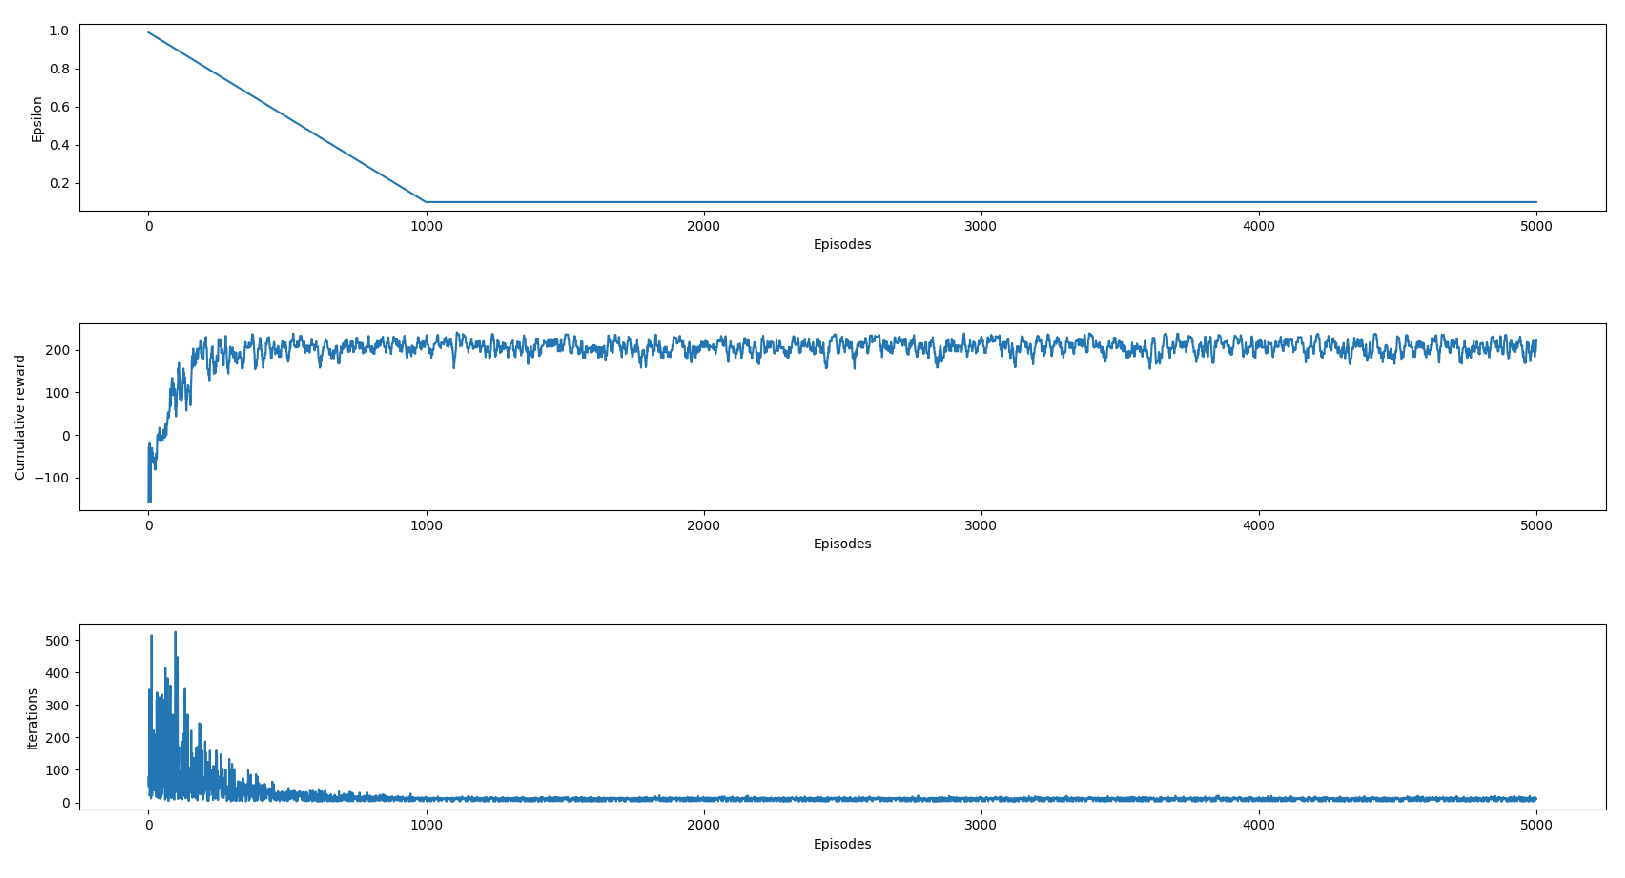
\includegraphics[height=8cm]{imagenes/cap4/14_training_graph.png}
    \end{center}
    \caption[Gráfico de entrenamiento]{Gráfico de entrenamiento}
    \label{fig:training_graph}
\end{figure}

Por último, se muestran los gráficos comparativos que nos dan un aproximado del \textbf{rendimiento} de cada algoritmo. En este caso, también se analizan tres cosas: el \textbf{tiempo medio} en segundos que tarda el dron desde que despega hasta que vuelve a su posición de despegue; el \textbf{número medio de iteraciones} empleadas para alcanzar la señal; y el \textbf{número medio de movimientos} hacía coordenadas donde la señal es menor y no mayor\footnote[4]{Los datos arrojados han sido guardados en formato \emph{csv}.}.\\

\begin{figure} [H]
    \begin{center}
    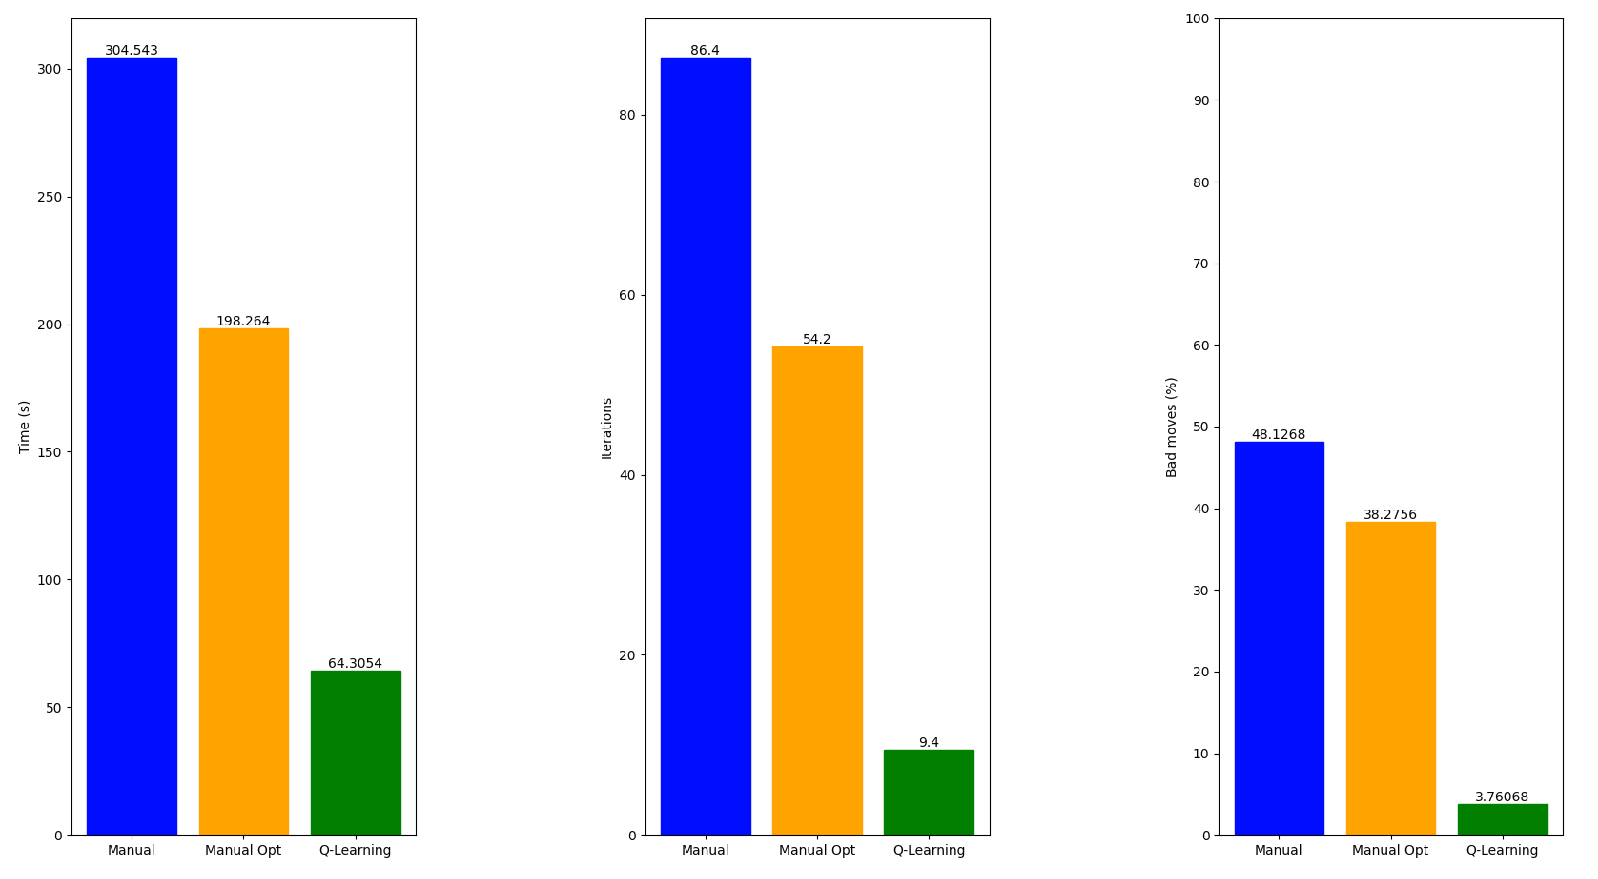
\includegraphics[height=8cm]{imagenes/cap4/15_avg_graphs.png}
    \end{center}
    \caption[Gráficos comparativos]{Gráficos comparativos}
    \label{fig:compare_graph}
\end{figure}

\subsection{Experimentos y resultados}
\label{subsec:experimentos_resultados}

Una vez sabemos que métricas se van a usar, queda ver que resultados arroja la experimentación. A excepción del último caso, las características de la señal siempre son los valores por defecto a excepción del tamaño del mapa, que se va modificando conforme el experimento. Además cabe destacar que la señal se toma como estática con respecto al dron, en posiciones diversas, también según el experimento a realizar.\\

\begin{figure} [H]
    \begin{center}
    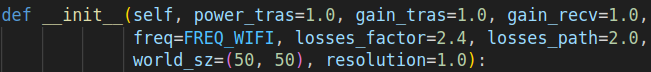
\includegraphics[height=1cm]{imagenes/cap4/16_default_values.png}
    \end{center}
    \caption[Características de la señal por defecto]{Características de la señal por defecto}
    \label{fig:compare_graph}
\end{figure}

Primero se probó sobre un escenario de tamaño \textbf{12x12 metros}, donde se distinguen dos posiciones de señal, una centrada y otra cerca de una esquina.\\
\newpage
Para la \textbf{señal cerca del centro}, se dispuso en las coordenadas (5, 5) del \emph{``heatmap''}, siguiendo el siguiente mapa de puntos para los puntos de entrenamiento e inferencia:\\

\begin{figure} [H]
    \begin{center}
    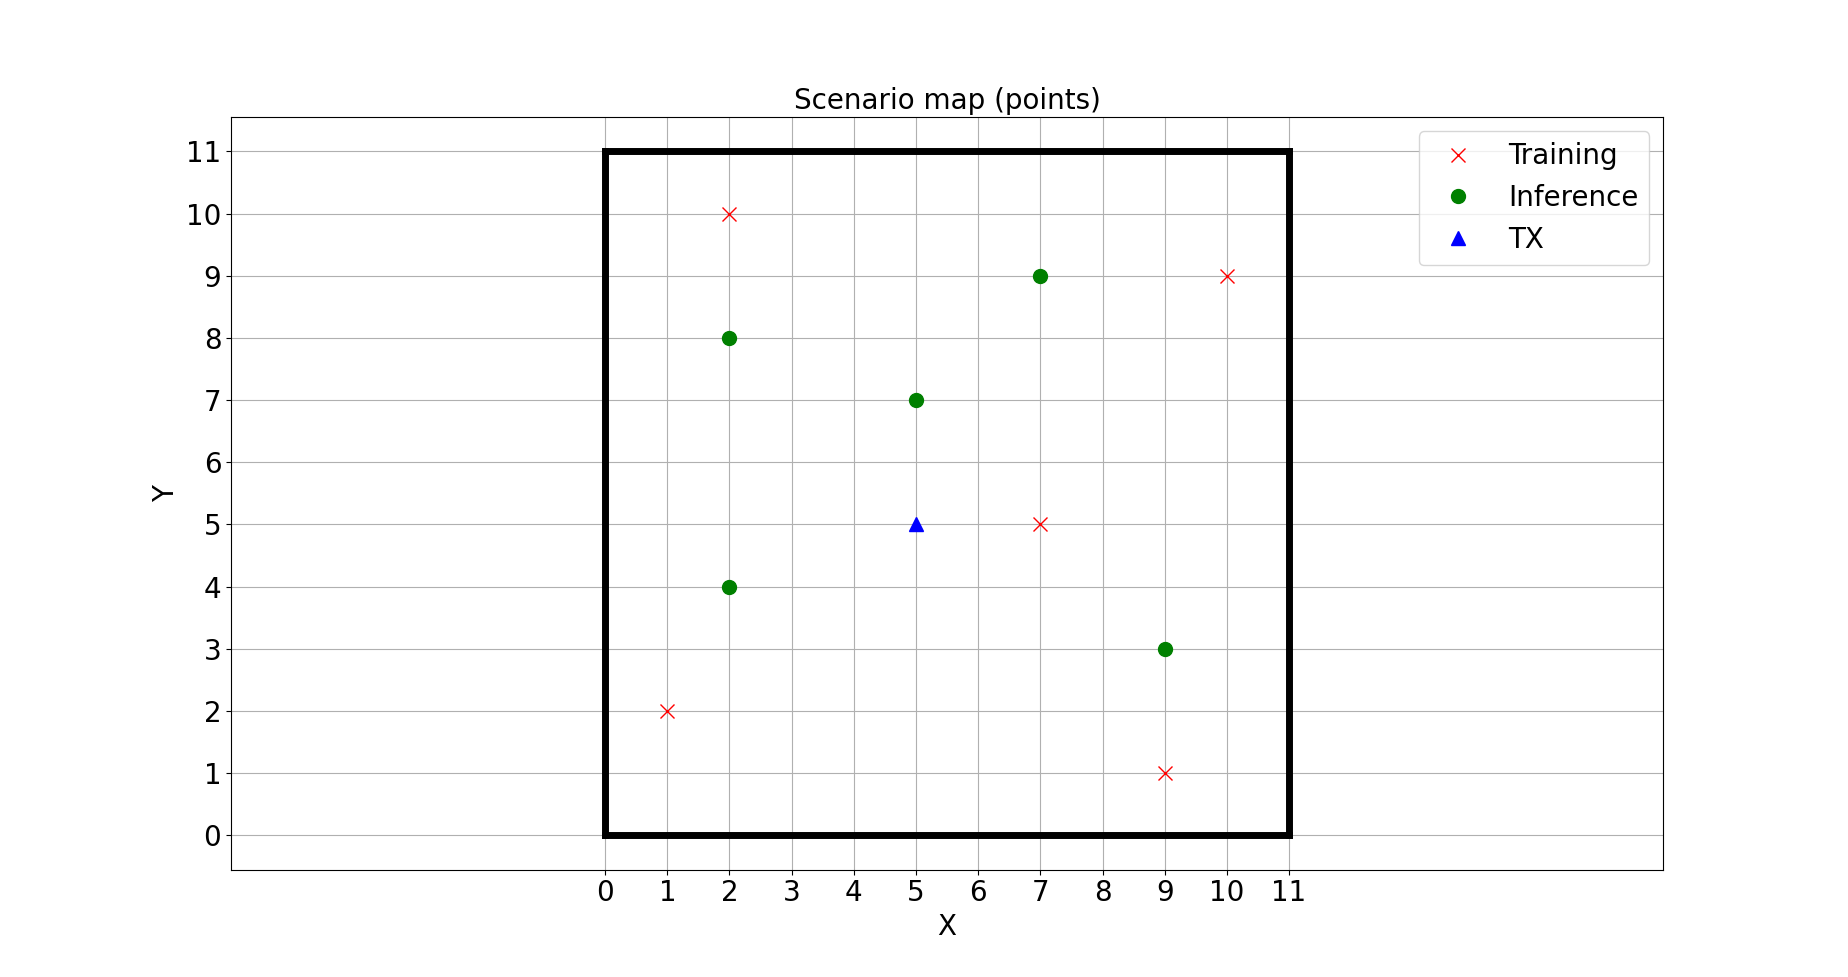
\includegraphics[height=8cm]{imagenes/cap4/17_mapa_p_centro_12.png}
    \end{center}
    \caption[Mapa de puntos (12x12), señal centrada]{Mapa de puntos (12x12), señal centrada}
    \label{fig:map_p_center_12}
\end{figure}

Los resultados obtenidos arrojan que el algoritmo más eficiente es el de Q-Learning, ya que tarda menos tiempo, realiza menos iteraciones hasta llegar a la meta y tiene un porcentaje inferior de malas acciones, tal y como podemos ver a continuación:\\

\begin{figure} [H]
    \begin{center}
    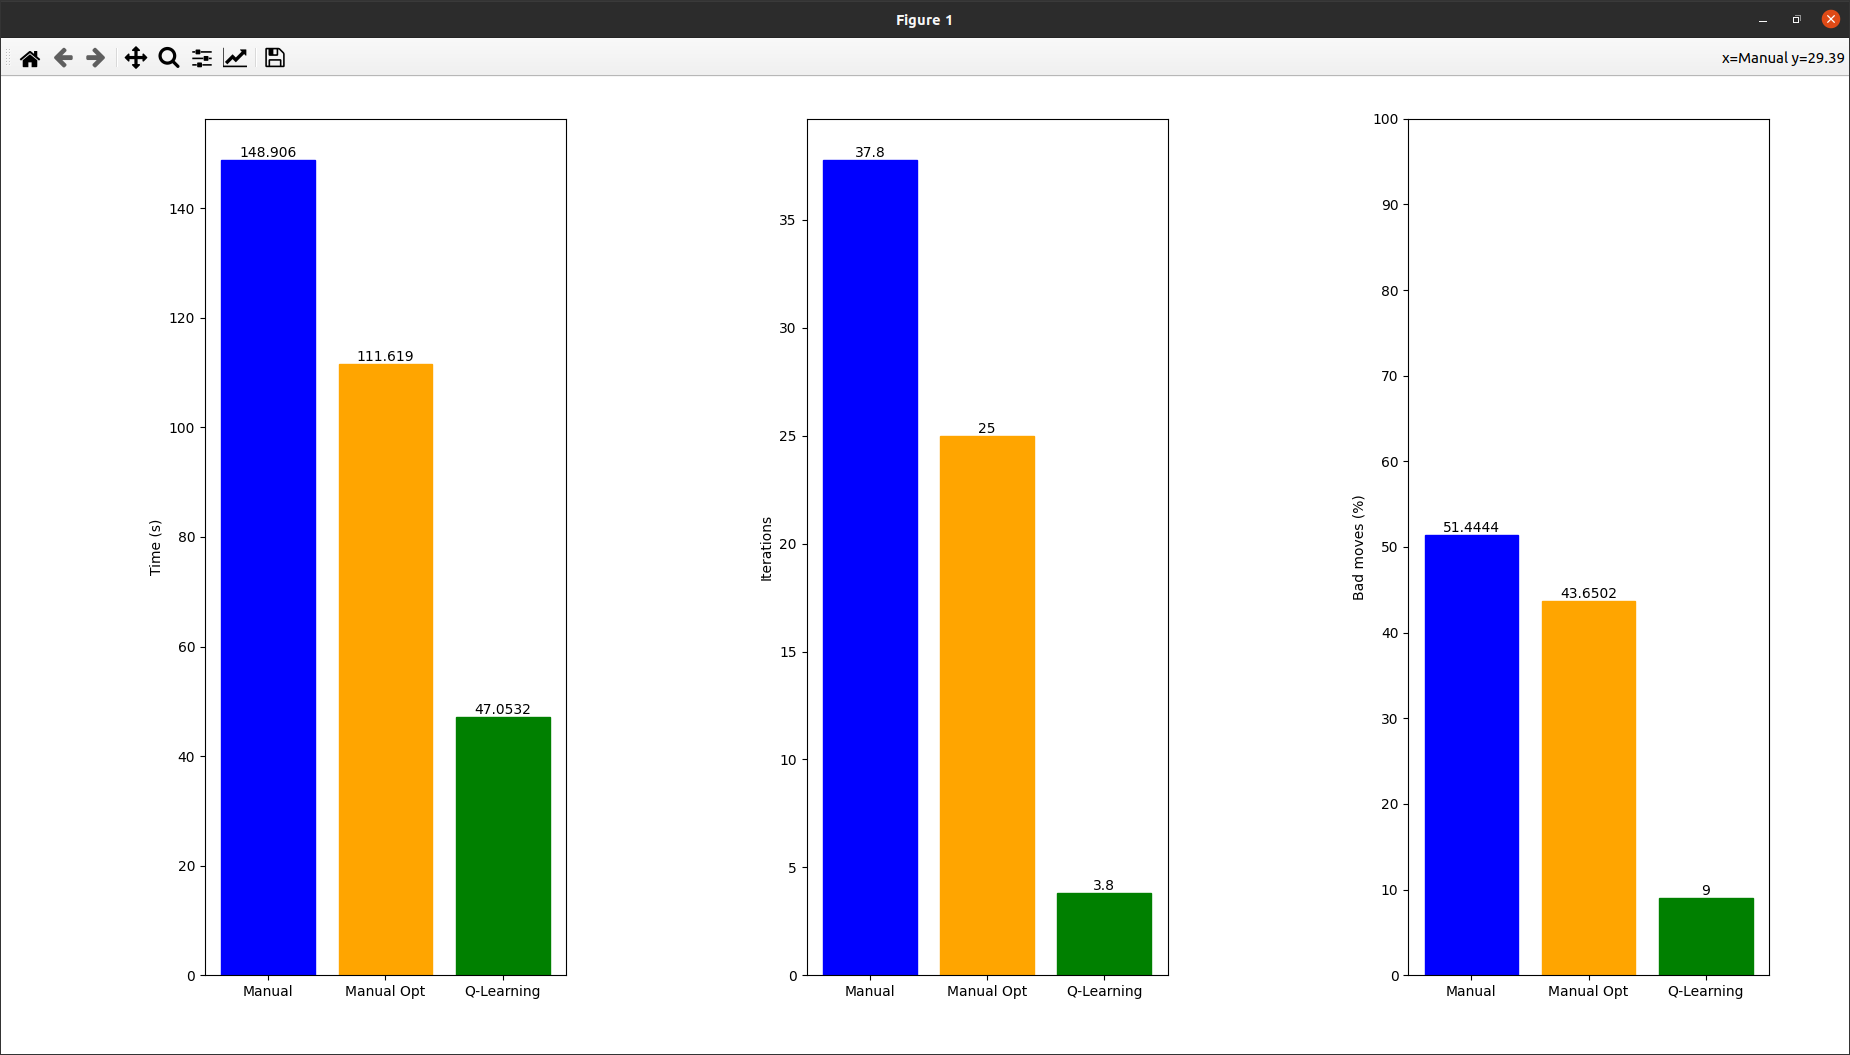
\includegraphics[height=8cm]{imagenes/cap4/18_comp_centro_12.png}
    \end{center}
    \caption[Comparativas (12x12), señal centrada]{Comparativas (12x12), señal centrada}
    \label{fig:comp_center_12}
\end{figure}

En el caso de la \textbf{señal cerca de la esquina}, la señal se estableció en (3, 1) referente a las coordenadas del \emph{``heatmap''}, siendo su mapa de puntos el siguiente:

\begin{figure} [H]
    \begin{center}
    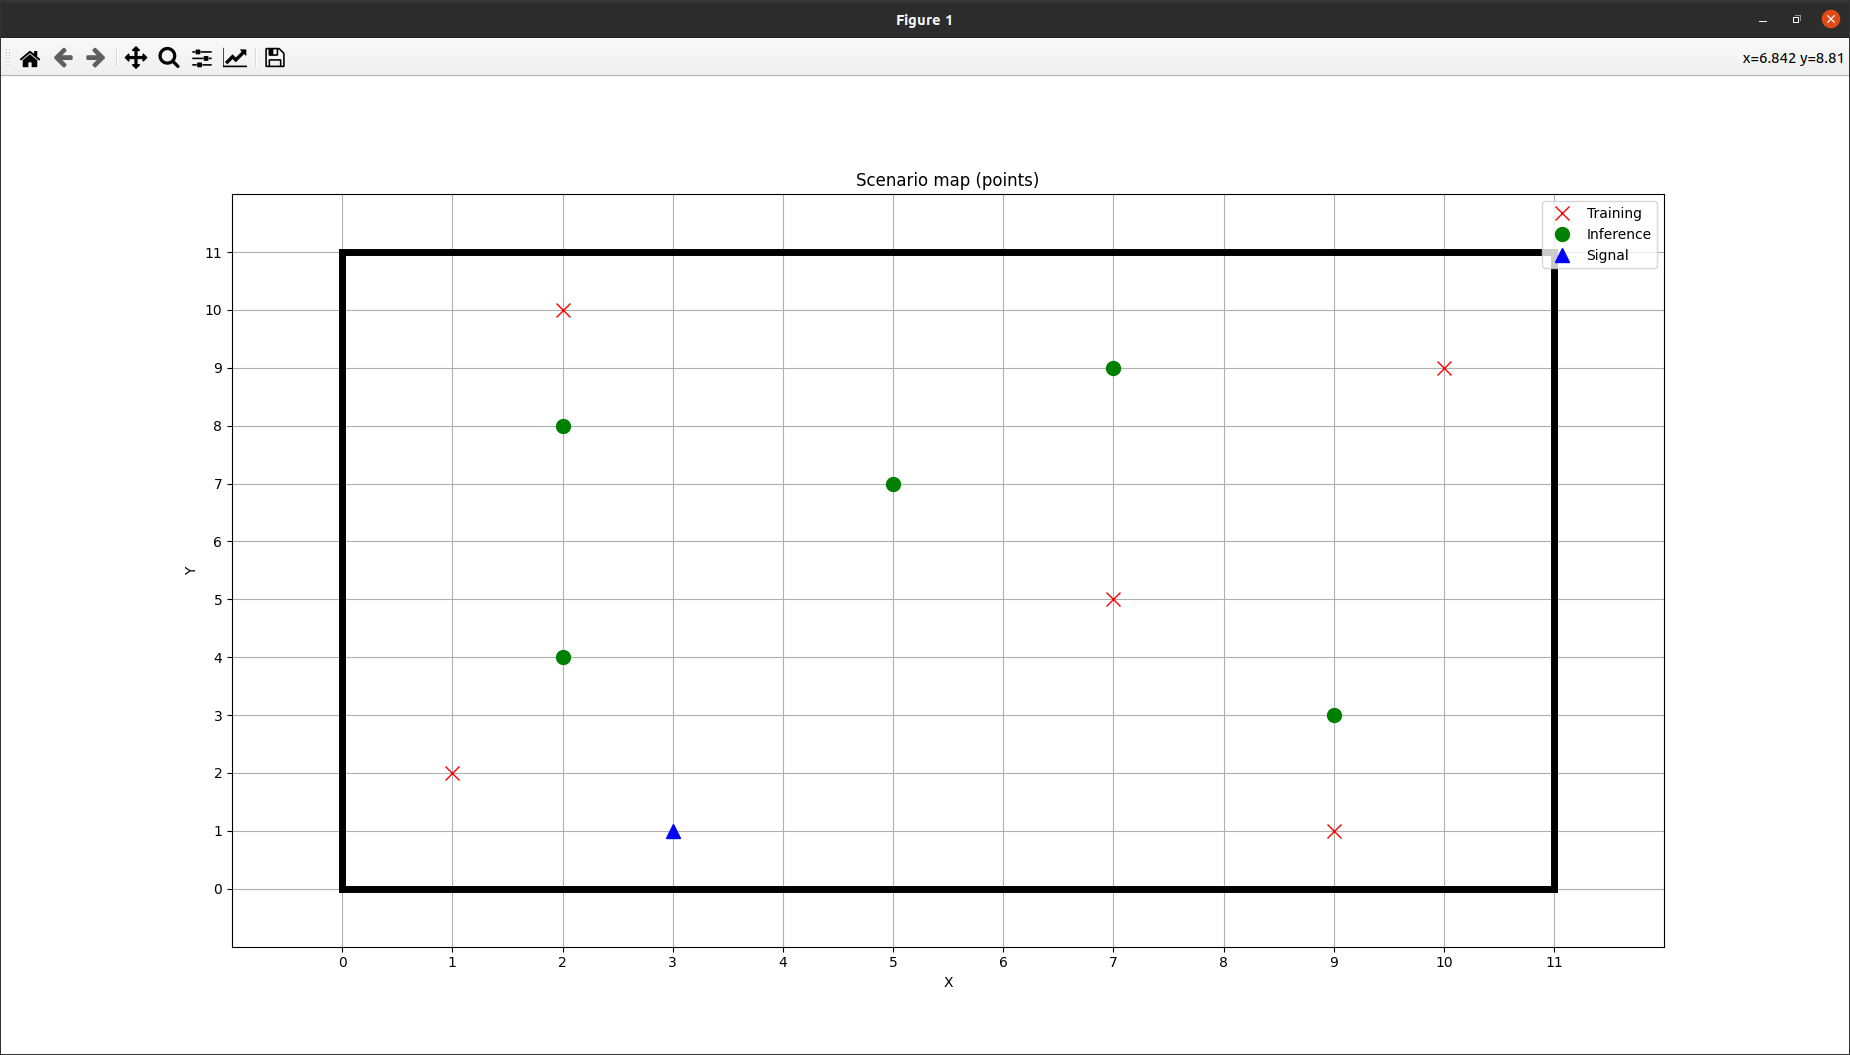
\includegraphics[height=8cm]{imagenes/cap4/19_mapa_p_esq_12.png}
    \end{center}
    \caption[Mapa de puntos (12x12), señal en la esquina]{Mapa de puntos (12x12), señal en la esquina}
    \label{fig:map_p_esq_12}
\end{figure}

En este caso, se obtiene la misma conclusión que en el escenario anterior, tal y como se puede apreciar a continuación:\\

\begin{figure} [H]
    \begin{center}
    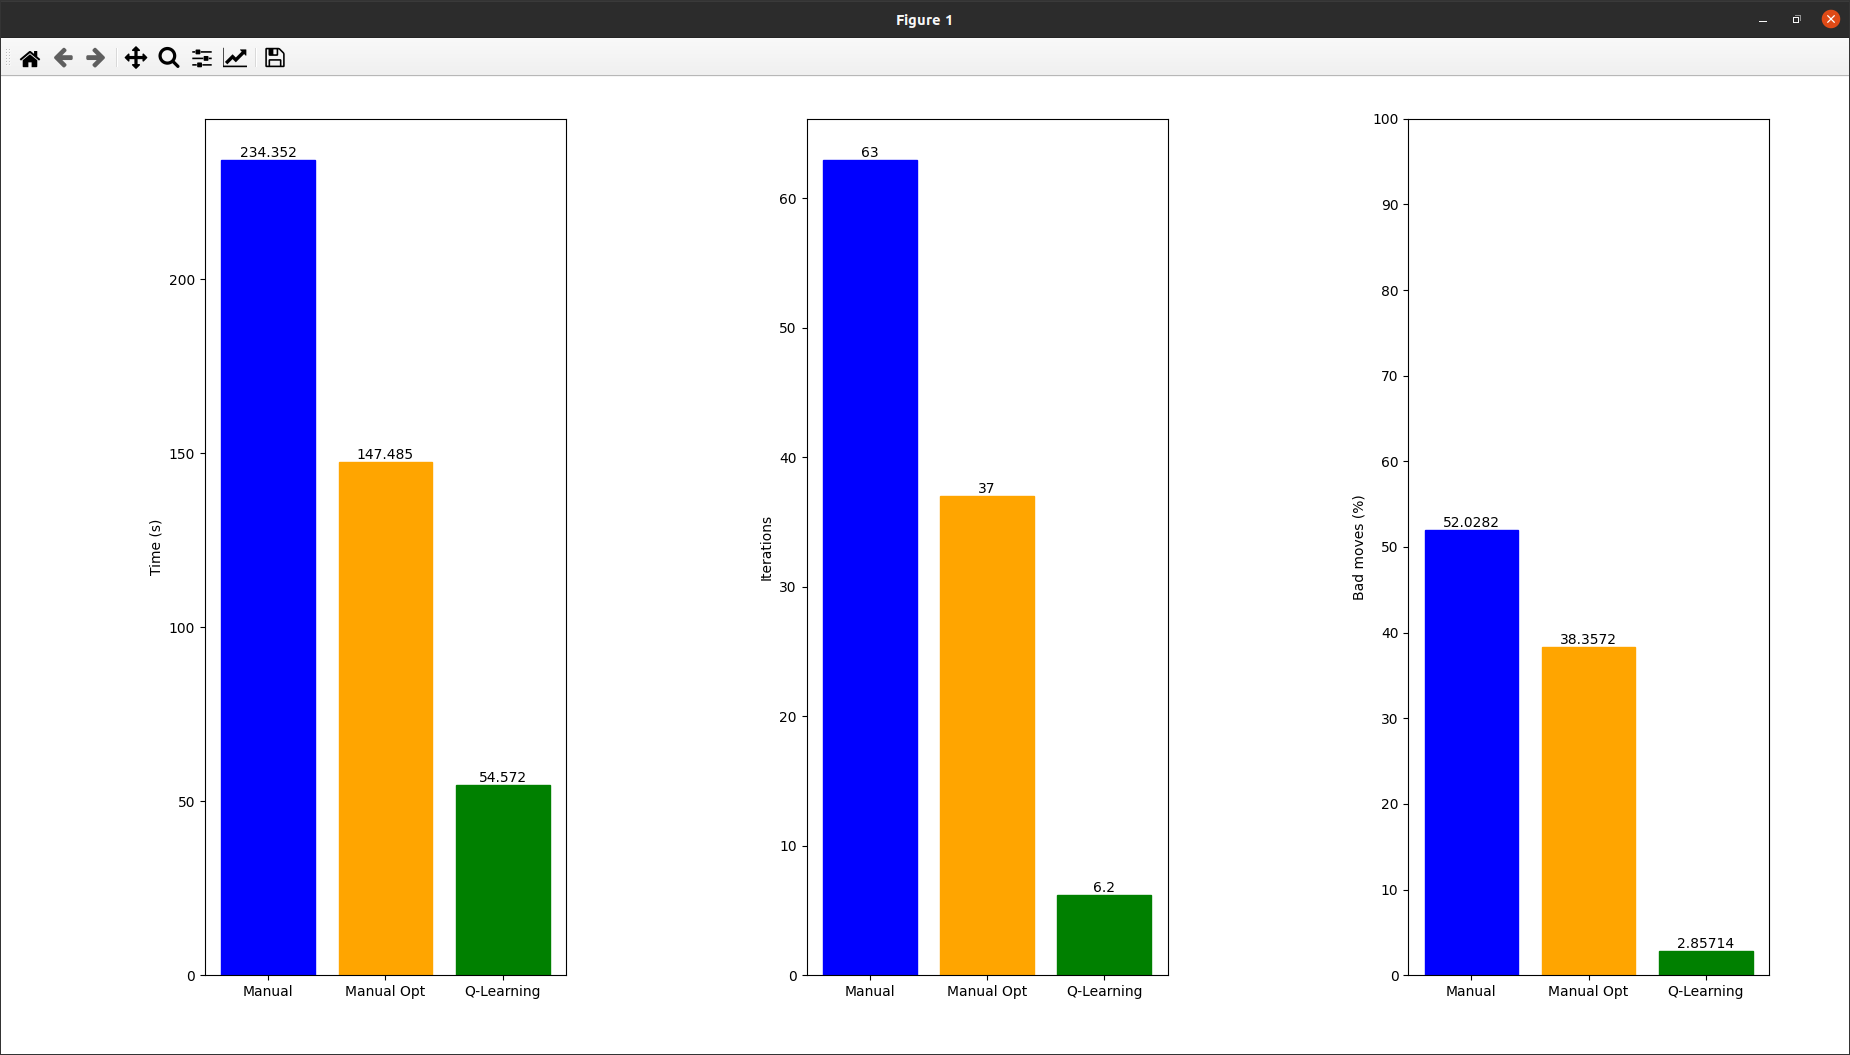
\includegraphics[height=8cm]{imagenes/cap4/20_comp_esq_12.png}
    \end{center}
    \caption[Comparativas (12x12), señal en la esquina]{Comparativas (12x12), señal en la esquina}
    \label{fig:comp_esq_12}
\end{figure}
\newpage
En segundo lugar, se incrementó el tamaño del mapa hasta \textbf{30x30 metros}.\\

Nuevamente, para la \textbf{señal cerca del centro} en (12, 12):

\begin{figure} [H]
    \begin{center}
    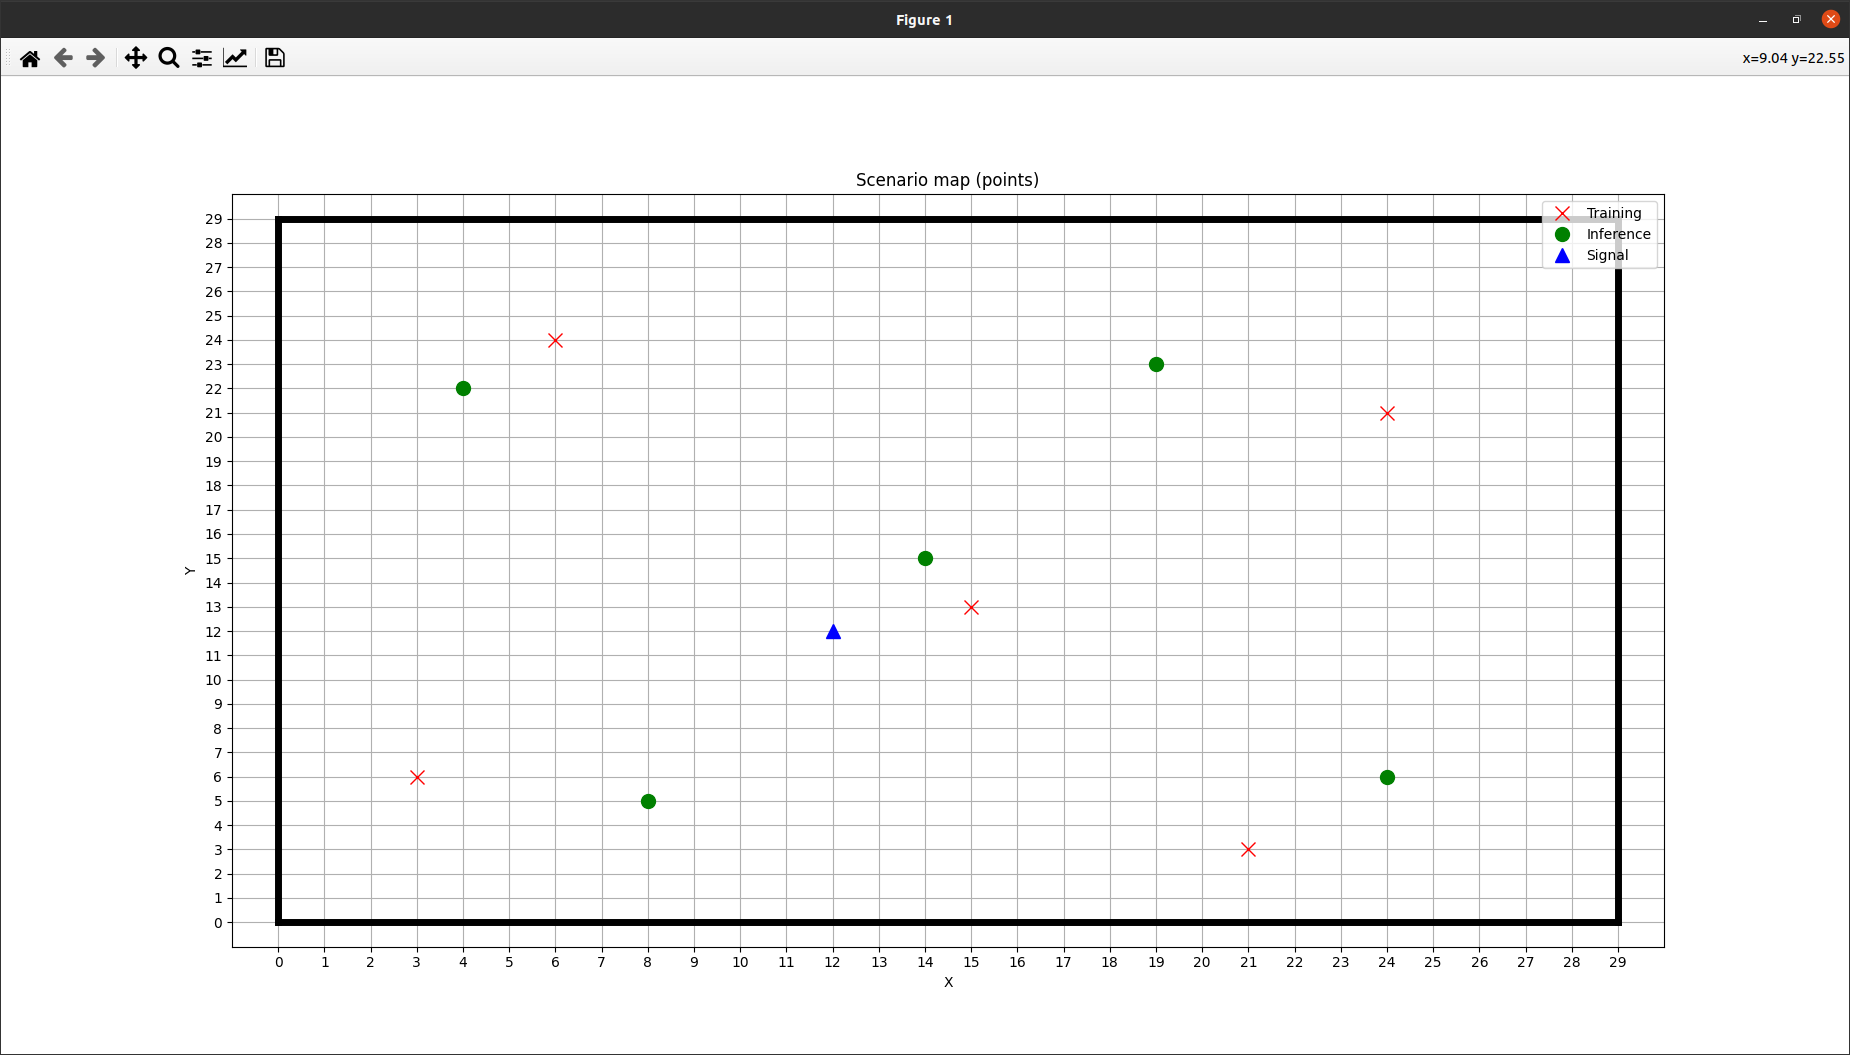
\includegraphics[height=8cm]{imagenes/cap4/21_mapa_p_centro_30.png}
    \end{center}
    \caption[Mapa de puntos (30x30), señal centrada]{Mapa de puntos (30x30), señal centrada}
    \label{fig:map_p_center_30}
\end{figure}

En cuanto a los resultados, concluimos que Q-Learning vuelve a ser la mejor opción, que aunque se vea un incremento temporal y de iteraciones por el aumento de mapa, sigue superando al resto:\\

\begin{figure} [H]
    \begin{center}
    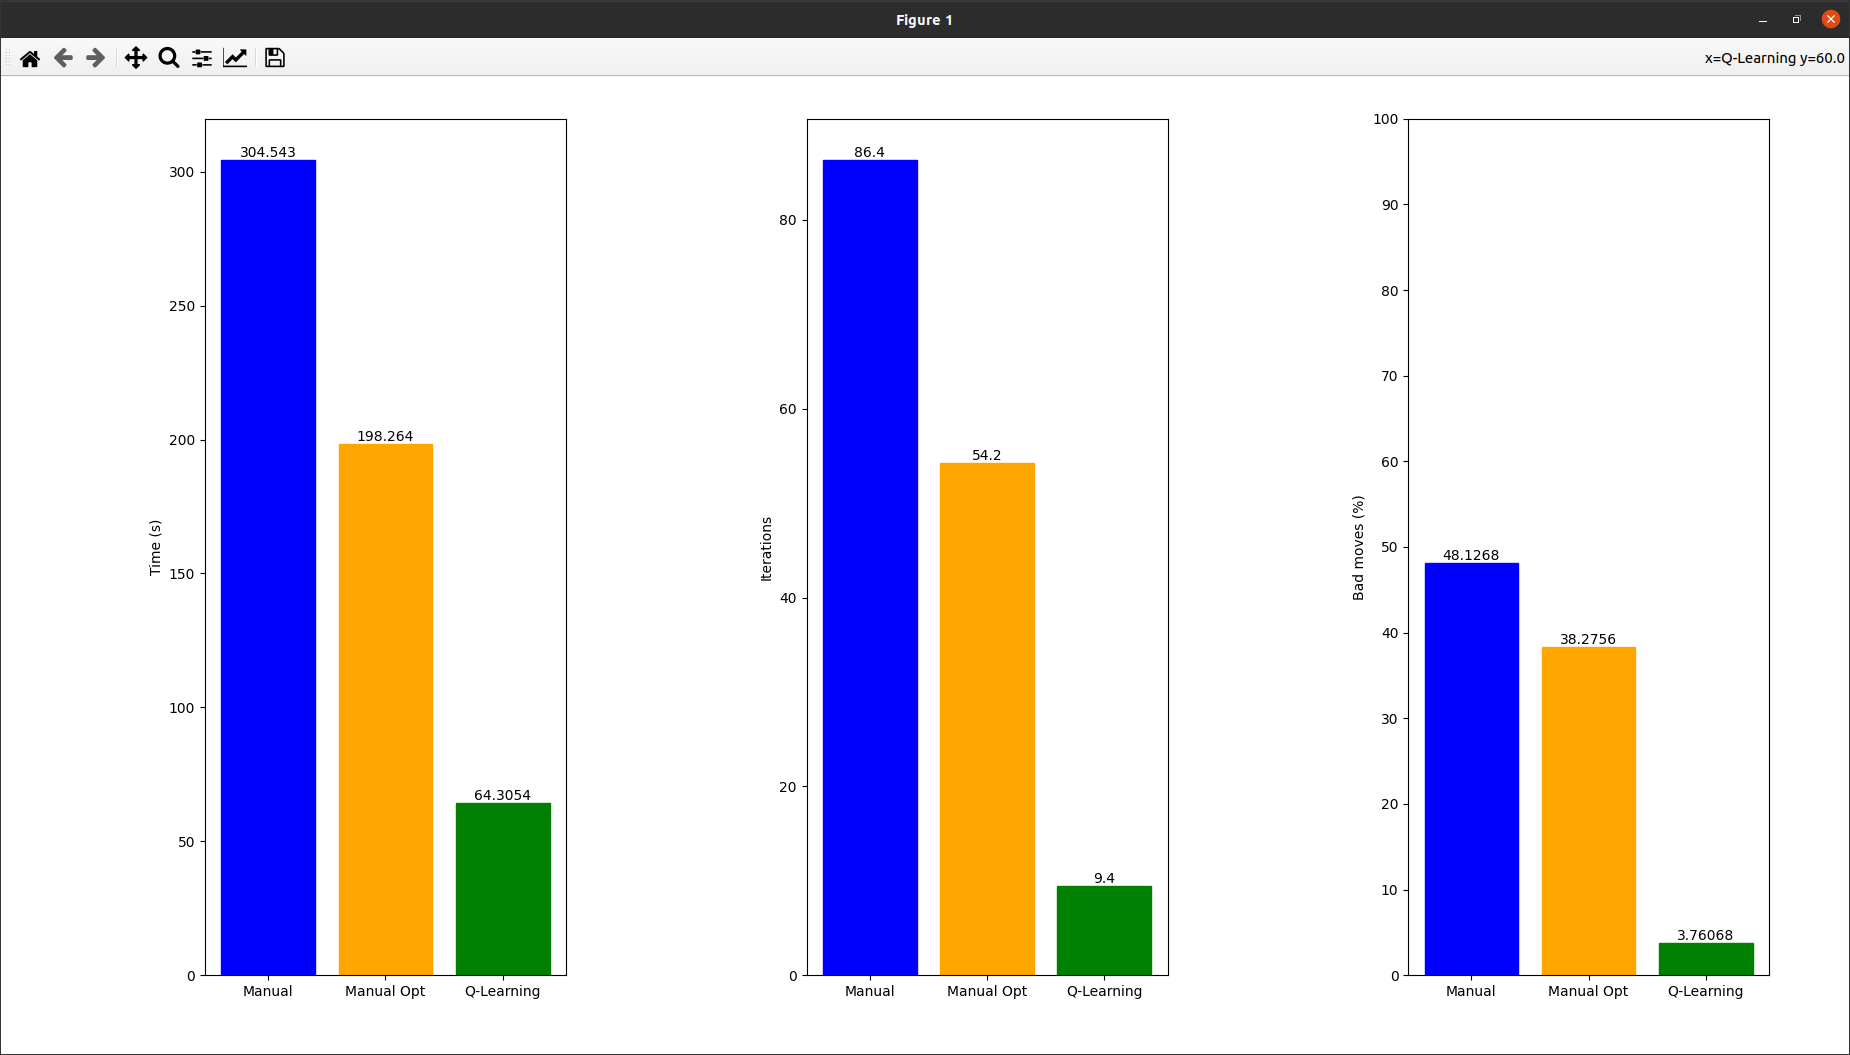
\includegraphics[height=8cm]{imagenes/cap4/22_comp_centro_30.png}
    \end{center}
    \caption[Comparativas (30x30), señal centrada]{Comparativas (30x30), señal centrada}
    \label{fig:comp_center_30}
\end{figure}

Continuando con la \textbf{señal cerca de la esquina}, en este caso se encuentra en las coordenadas (5, 3), y su mapa de puntos es:\\

\begin{figure} [H]
    \begin{center}
    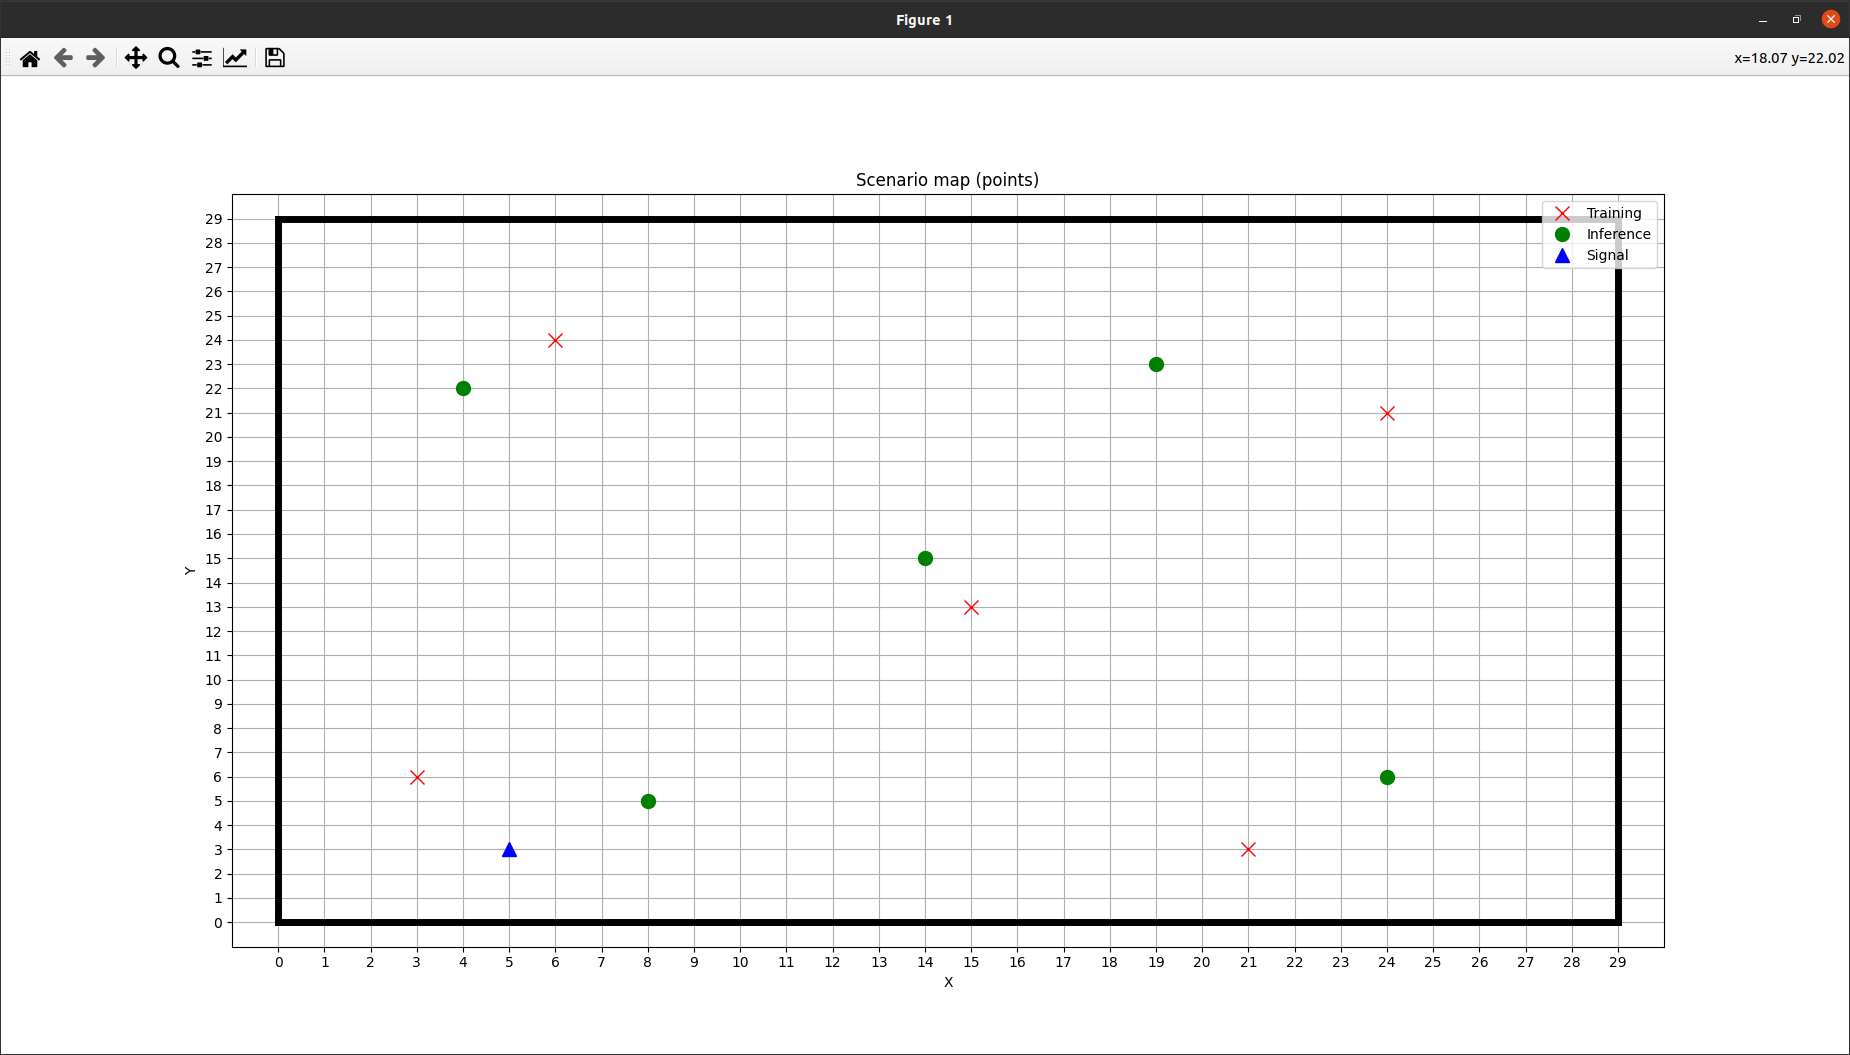
\includegraphics[height=8cm]{imagenes/cap4/23_mapa_p_esq_30.png}
    \end{center}
    \caption[Mapa de puntos (30x30), señal en la esquina]{Mapa de puntos (30x30), señal en la esquina}
    \label{fig:map_p_esq_30}
\end{figure}

De igual modo vemos que el resultado de aprendizaje por refuerzo es claramente superior:\\

\begin{figure} [H]
    \begin{center}
    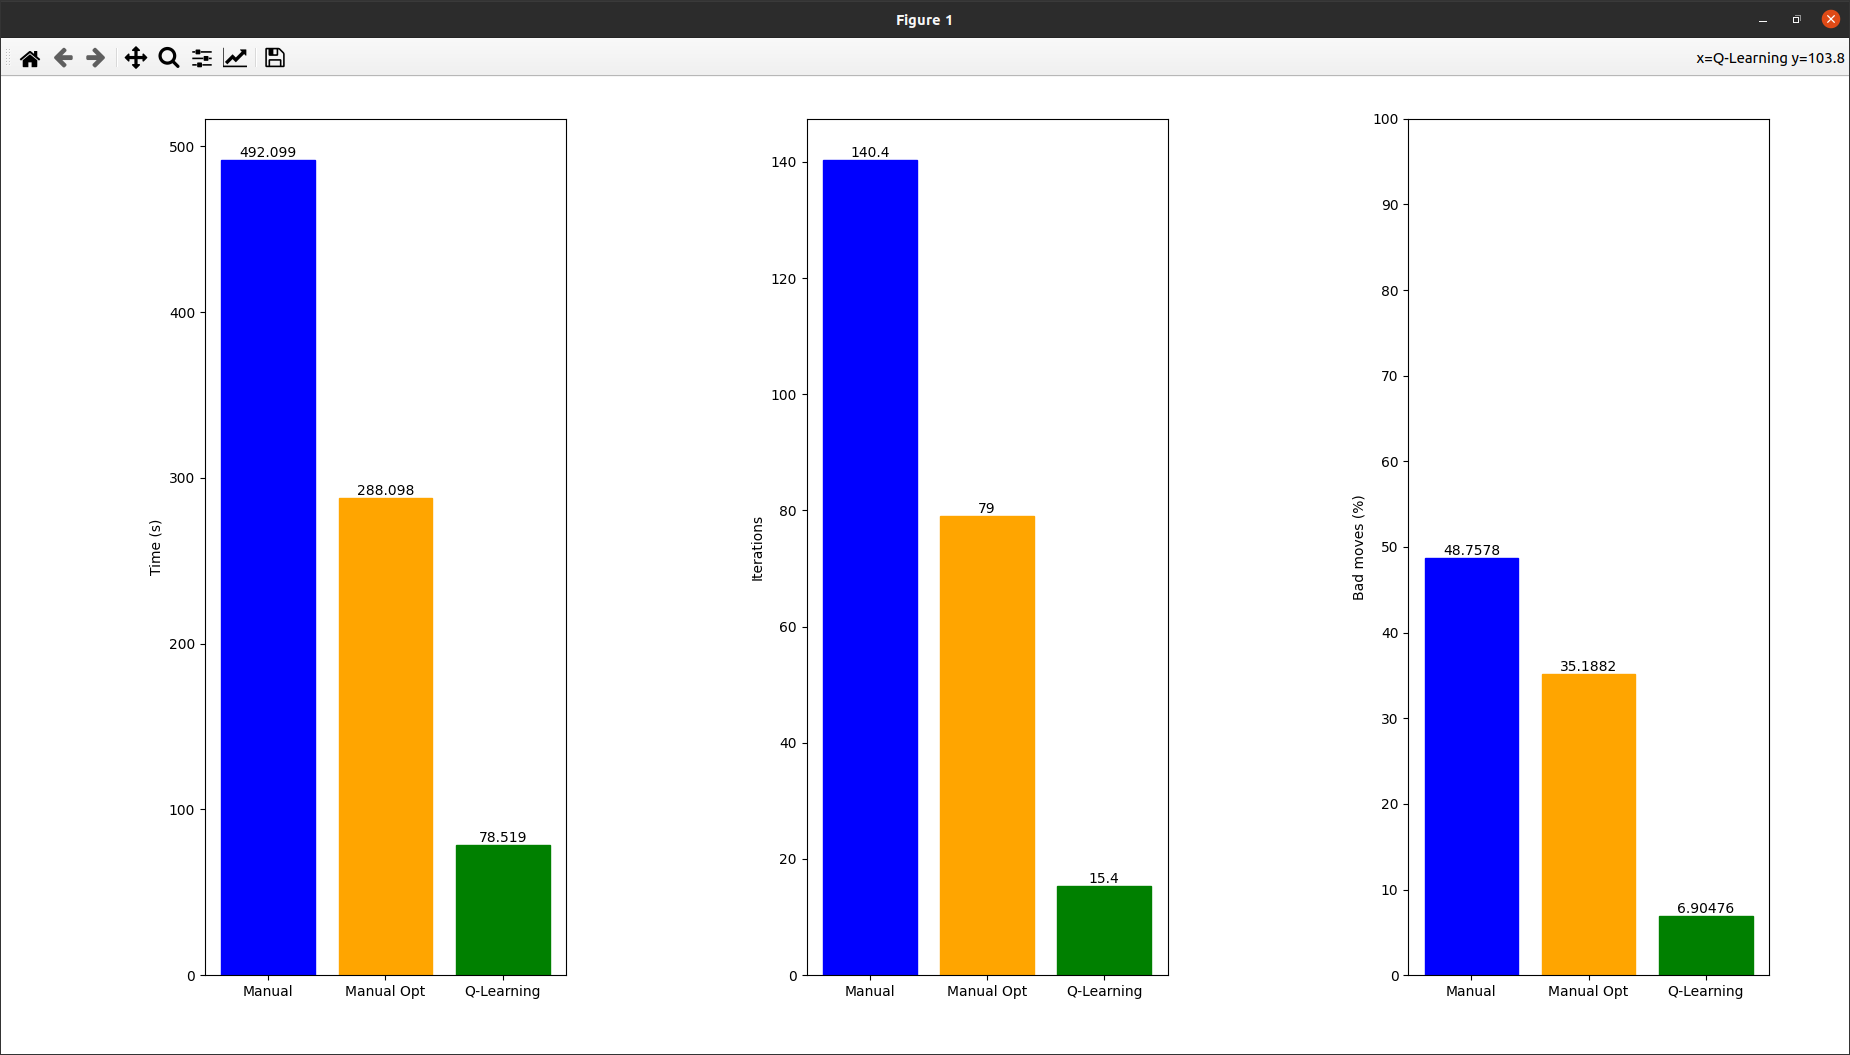
\includegraphics[height=8cm]{imagenes/cap4/24_comp_esq_30.png}
    \end{center}
    \caption[Comparativas (30x30), señal en la esquina]{Comparativas (30x30), señal en la esquina}
    \label{fig:comp_esq_30}
\end{figure}
\newpage
Por último, se planteó un problema sólo para Q-Learning, en el cual se \textbf{entrenaba al modelo con una señal}, y se \textbf{realizaba inferencia con otra señal con características distintas}, aumentando la potencia del transmisor al doble y cambiando la frecuencia para simular una señal 5G, situada en (5, 3):\\

\begin{figure} [H]
    \begin{center}
    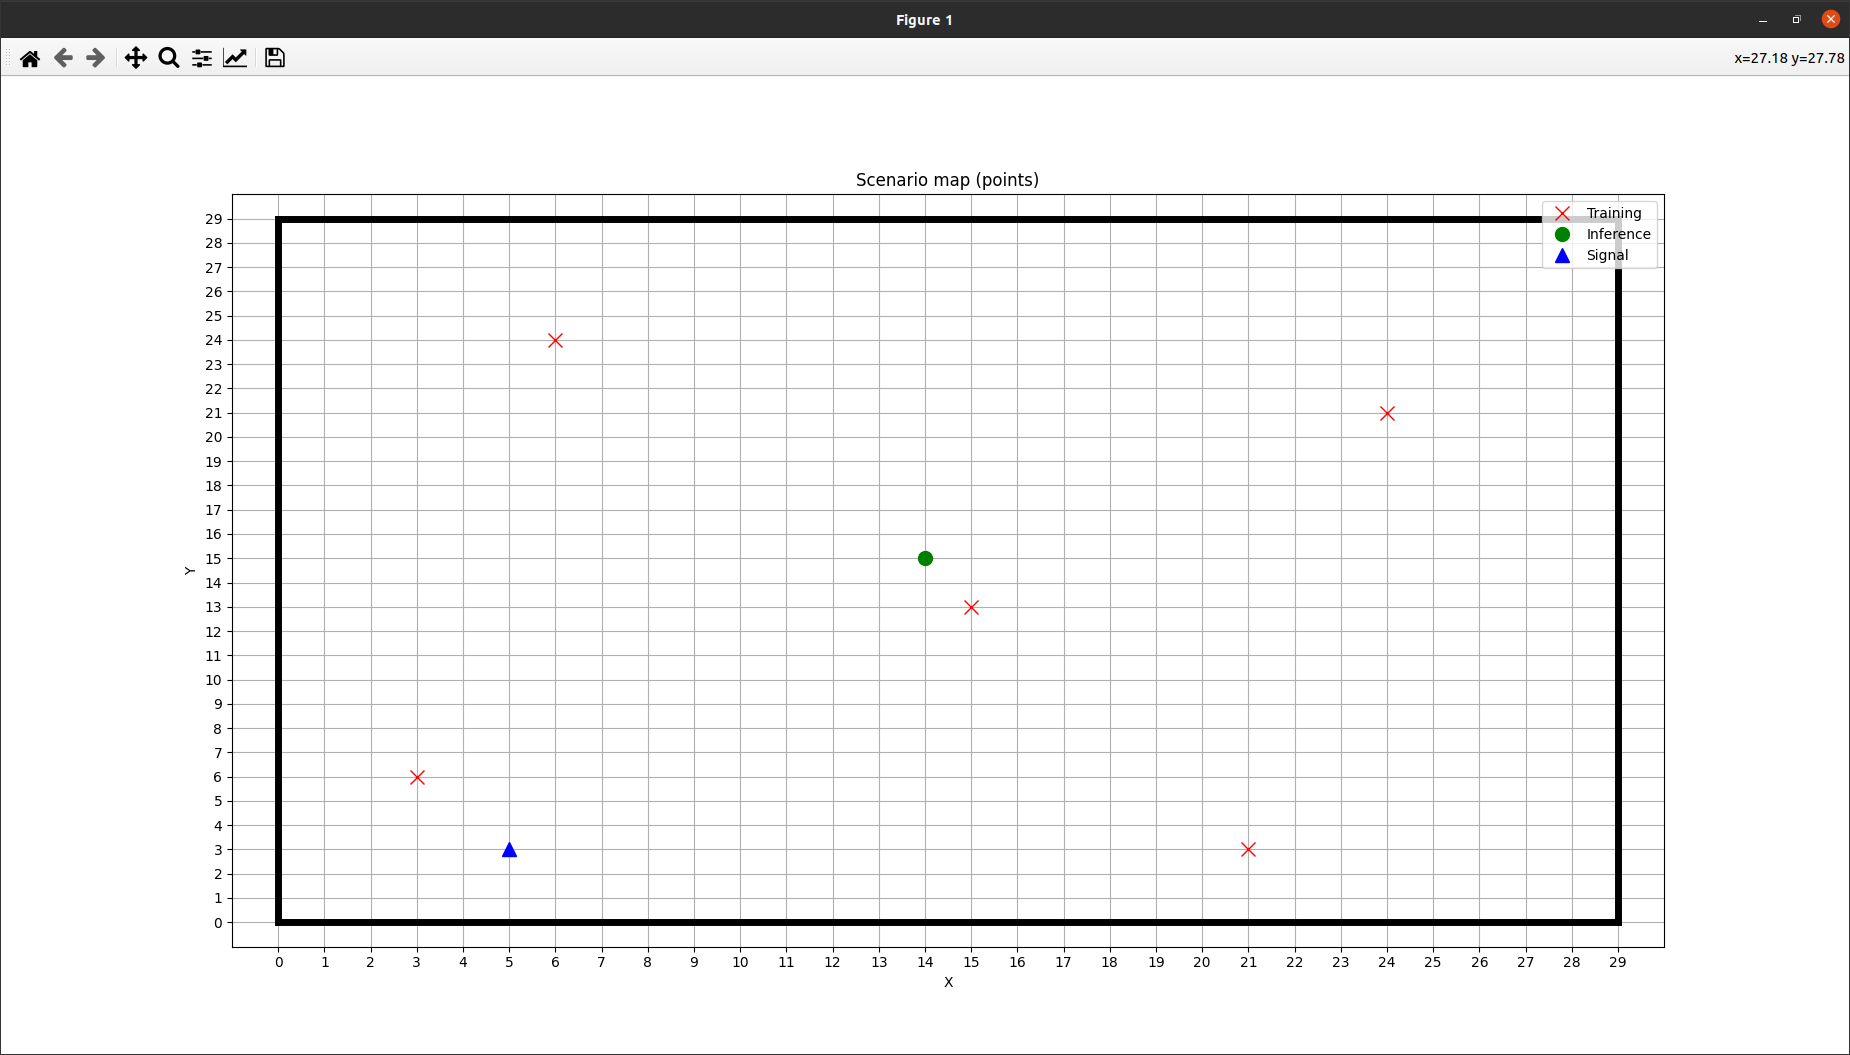
\includegraphics[height=8cm]{imagenes/cap4/25_mapa_p_diff.png}
    \end{center}
    \caption[Mapa de puntos (30x30), señales diferentes]{Mapa de puntos (30x30), señales diferentes}
    \label{fig:map_p_diff_30}
\end{figure}

Para este caso, el problema se resolvía de igual forma para ambos casos, con una cierta variación en el tiempo, derivada probablemente de la propia simulación:\\

\begin{figure} [H]
    \begin{center}
    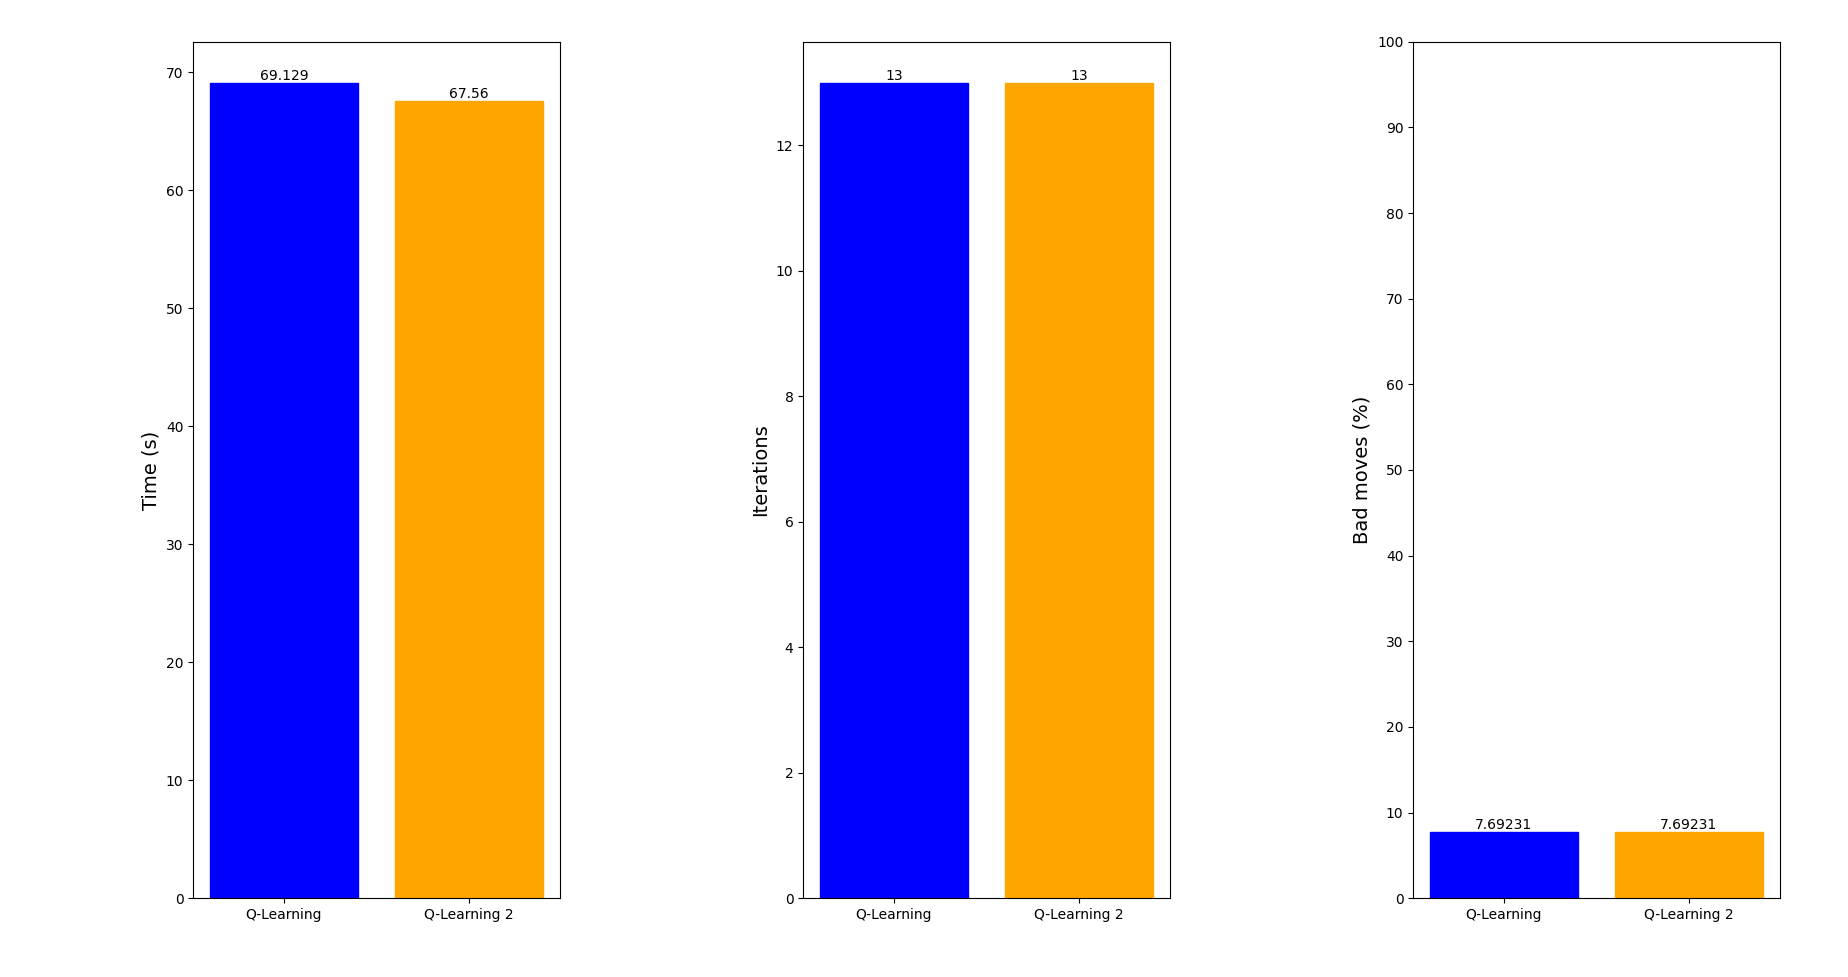
\includegraphics[height=7.5cm]{imagenes/cap4/26_comp_diff.png}
    \end{center}
    \caption[Comparativas (30x30), señales diferentes]{Comparativas (30x30), señales diferentes}
    \label{fig:comp_diff_30}
\end{figure}

\subsection{Líneas a futuro - Experimentos con obstáculos}
\label{subsec:experimentos_obstaculos}

El escenario planteado durante el \ac{TFG}, al fin y al cabo, es la aproximación más simple, es decir, en un \textbf{caso real} no es esperable un entorno vacío de perturbaciones y obstáculos. Por ello, el siguiente paso lógico es \textbf{implementar muros que distorsionen la señal} y ver como se comporta con Q-Learning.\\

Para ello, la idea es conseguir modificar el módulo de Friis, para que pueda agregar de forma dinámica obstáculos al mapa, empleando un algoritmo que identifica si los puntos se encuentran dentro del polígono generado por las proyecciones de la señal, con los vértices del muro \cite{poly-info}. Posteriormente se degrada la señal usando un factor de pérdidas.\\

\begin{figure} [H]
    \begin{center}
    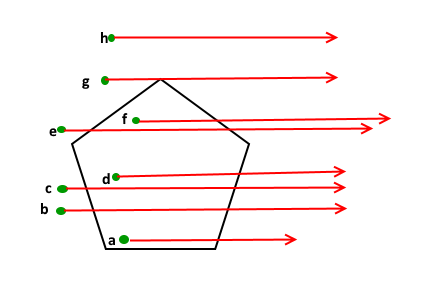
\includegraphics[height=6cm]{imagenes/cap4/27_points_poly.png}
    \end{center}
    \caption[Funcionamiento del algoritmo de puntos]{Funcionamiento del algoritmo de puntos}
    \label{fig:poly_algorithm}
\end{figure}

Para las primeras pruebas, se estableciieron a mano los valores degradados de la señal, sobre un mapa con obstáculos.\\

Además, la idea inicial era realizar el entrenamiento \textbf{sin obstáculos}, y ajustar los algoritmos para que fueran capaces de sortear los mismos.\\
\newpage
De este modo, y cómo primera aproximación a este proceso, se distinguieron \textbf{dos casos}:

\begin{enumerate}
    \item \emph{El dron vuela por encima de la altura del obstáculo}: En cuyo caso se ve que es capaz de navegar satisfactoriamente hacia la señal, con las soluciones empleadas previamente.

    \item \emph{El dron vuela a la misma altura que el obstáculo}: Donde se observa que la solución de Q-Learning queda insuficiente para resolver el problema, ya que el dron colisiona directamente con el obstáculo. Por ello, se plantea la idea de agregar un sistema de detección (o sensor) que permita al dron sortear los muros. Para el caso simulado simplemente se comprueba si la siguiente posición corresponde a un obstáculo en el mapa de calor y se actúa en consecuencia. Sin embargo, seguimos trabajando en este apartado.
\end{enumerate}

\begin{figure} [H]
    \begin{center}
    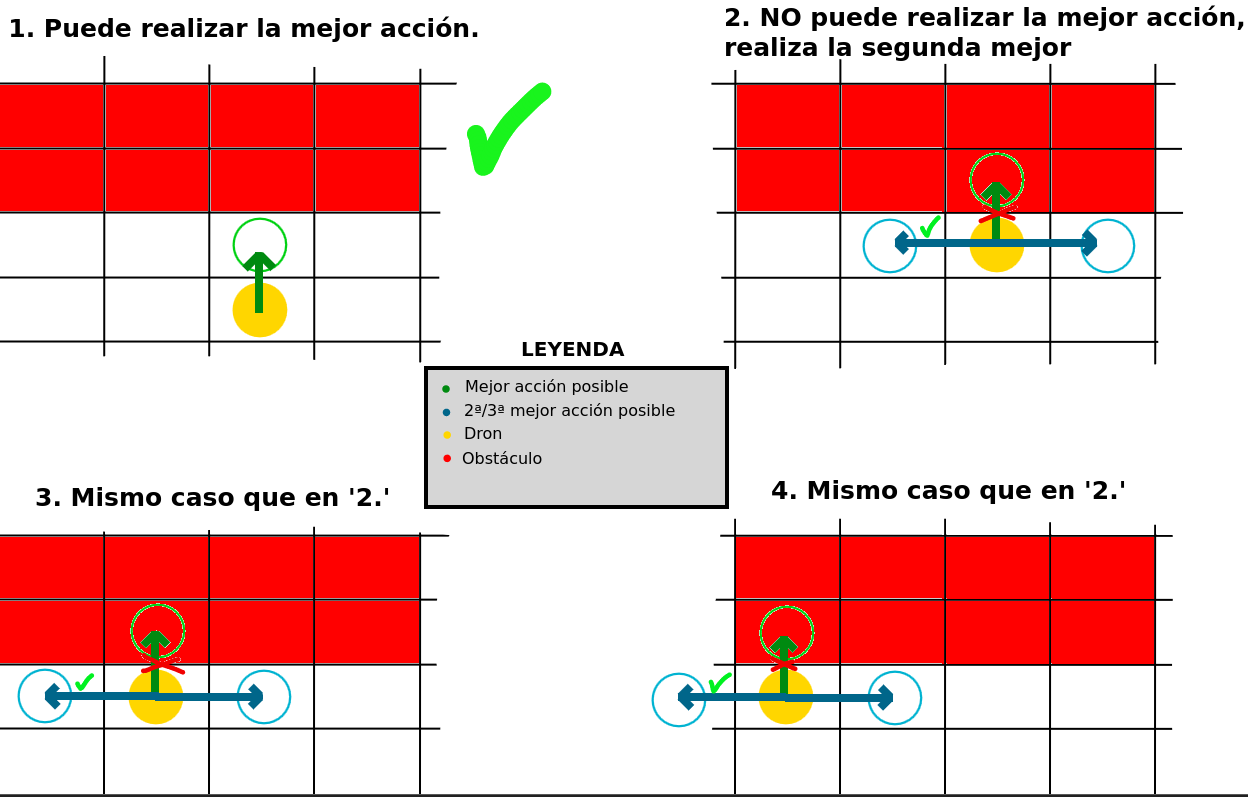
\includegraphics[height=9cm]{imagenes/cap4/28_pseudosensor.png}
    \end{center}
    \caption[Simulación de sensor para obstáculo]{Simulación de sensor para obstáculo}
    \label{fig:pseudosensor}
\end{figure}

\chapter{Conclusiones}
\label{cap:capitulo5}

ToDo...

\section{Objetivos cumplidos}
\label{sec:objetivos_cumplidos}

ToDo...

\section{Requisitos satisfechos}
\label{sec:requisitos_satisfechos}

ToDo...

\section{Balance global y competencias adquiridas}
\label{sec:balance_global_competencias_adquiridas}

ToDo...

\section{Líneas futuras}
\label{sec:lineas_futuras}

ToDo...

\chapter*{Anexo}
\label{cap:anexo}

A continuación muestro una serie de conceptos básicos relacionados con el estudio del procesamiento de señales\footnote[1]{Información extraida de la siguiente colección de videos didácticos \url{https://www.youtube.com/playlist?list=PL8bSwVy8_IcPCsBE71CYBLbQSS8ckWm6x}}:

\begin{enumerate}
	\item \emph{Señal}: se trata de una función que describe un fenómeno físico, y que se emplea para la transmisión de información.
    \item \emph{Dominio temporal}: establece el eje de abcisas con el tiempo.
    \item \emph{Dominio de la señal}: determina si la señal se expresa en tiempo o en frecuencia (a través de transformadas).
    \item \ac{ADC}: elemento electrónico que permite la conversión de señales analógicas a señales digitales.
    \item \ac{RSSI}: permite establecer el nivel de potencia de una señal, con respecto a 1 mW de potencia. Se expresa en dBm.
    \item \ac{SNR}: métrica que permite medir la potencia de la señal con respecto al ruido ambiente.
    \item \emph{Frecuencia}: parámetro de la función que define a la señal, el cual determina el número de veces que se repite en un segundo. Se mide en hercios (Hz).
    \item \emph{TX}: Se refiere a la transmisión de la señal.
    \item \emph{RX}: Hace referencia a la recepción de la señal.
\end{enumerate}

\printindex \nocite{*}
\appendix

\bibliographystyle{unsrt}

\bibliography{bibliografia}

\end{document}
